\documentclass[a4paper,12pt]{article}
\usepackage{geometry}
\usepackage{amsmath,amsfonts,amssymb}
\usepackage{graphicx}
\usepackage{subcaption}
\usepackage{caption}
\usepackage{booktabs}
\usepackage{hyperref}
\usepackage{enumitem}
\usepackage{xcolor}
\usepackage{titling}
\usepackage{fancyhdr}
\usepackage{parskip}
\usepackage{listings}
\usepackage{float}
\usepackage{tikz}
\usetikzlibrary{arrows.meta,positioning}

% Custom colors
\definecolor{titleblue}{RGB}{0,102,204}
\definecolor{headingblue}{RGB}{0,51,102}

% Code listing style
\lstset{
    language=Python,
    basicstyle=\ttfamily\scriptsize,
    keywordstyle=\color{blue}\bfseries,
    stringstyle=\color{purple},
    commentstyle=\color{gray}\itshape,
    numberstyle=\tiny,
    numbers=left,
    stepnumber=1,
    numbersep=5pt,
    showspaces=false,
    showstringspaces=false,
    frame=single,
    breaklines=true,
    breakatwhitespace=true,
    tabsize=4
}

% Page layout
\geometry{top=2.5cm,bottom=2.5cm,left=2.5cm,right=2.5cm}
\setlength{\parindent}{0pt}
\setlength{\parskip}{0.8em}
\setlength{\headheight}{15pt}

% Header and footer
\pagestyle{fancy}
\fancyhf{}
\fancyhead[L]{\textbf{INS3155 - Computer Vision Midterm Report}}
\fancyhead[R]{Ha Manh Duc -- 23070287}
\fancyfoot[C]{\thepage}

% Title customization
\pretitle{\centering\LARGE\bfseries}
\posttitle{\par\vspace{0.5cm}}
\preauthor{\centering}
\postauthor{\par\vspace{0.3cm}}
\predate{\centering}
\postdate{\par}
\emergencystretch=3em

\hypersetup{colorlinks=true, linkcolor=headingblue, urlcolor=titleblue, citecolor=headingblue}

\tikzset{
    block/.style={rectangle, draw=headingblue, fill=titleblue!8, rounded corners=3pt,
                  minimum height=1.0cm, text width=2.1cm, align=center, font=\scriptsize},
    arrow/.style={-{Stealth[length=2.2mm]}, thick, headingblue}
}

\begin{document}

\title{\textcolor{titleblue}{Midterm Project Report}\\[0.3cm]
\large Traditional Image Processing for Filtering, 3D Reconstruction, and Image Stitching}

\author{\parbox{0.6\linewidth}{\centering
Name: Ha Manh Duc\\
Student ID: 23070287\\
Email: 23070287@vnu.edu.vn\\
Course: INS3155 -- Computer Vision}}

\date{November 2026}

\maketitle

\begin{abstract}
This report implements and systematically compares classical (non-learning) computer vision
methods on three tasks built from a custom architectural photograph. In \textbf{Part A}, Gaussian
($\sigma_n=25$) and salt-and-pepper (8\%) noise are removed with Mean, Gaussian, and Median filters and
enhanced with Laplacian sharpening over $3\times3$, $5\times5$ and $7\times7$ kernels; the $3\times3$ median
filter restores salt-and-pepper images from 15.83\,dB to 26.81\,dB PSNR (SSIM 0.928), while a
small Gaussian kernel is best for Gaussian noise (24.77\,dB). In \textbf{Part B}, the fundamental
matrix is estimated with SIFT and RANSAC (Sampson error 0.24\,px), and SGBM reduces disparity
RMSE by about 43\% compared to Block Matching against a known ground truth. In \textbf{Part C}, a
four-view panorama pipeline compares SIFT, ORB and AKAZE: SIFT and AKAZE reach sub-0.27\,px
reprojection RMSE, while ORB is roughly four times less accurate. Laplacian pyramid blending
and parameter sensitivity studies are included as extensions.
\end{abstract}

\tableofcontents
\newpage

%=====================================================================
\section{Introduction}
%=====================================================================
Classical image processing and multi-view geometry remain the backbone of many vision systems,
from camera image signal processors and document scanners to visual odometry and smartphone
panorama modes. Unlike deep networks, these methods are analytically interpretable, need no
training data, and run deterministically on a CPU, which makes them easy to reason about and to
benchmark. This project studies three such building blocks:

\begin{itemize}[leftmargin=*]
    \item \textbf{Image filtering (Part A):} denoising is the first stage of almost every pipeline;
          the key question is how to suppress noise without destroying edges.
    \item \textbf{Stereo 3D reconstruction (Part B):} recovering depth from two views underpins
          robotics, autonomous driving and photogrammetry; it requires epipolar geometry and dense
          correspondence.
    \item \textbf{Image stitching (Part C):} building panoramas tests feature detection, robust
          matching, homography estimation and blending in one end-to-end system.
\end{itemize}

For each task at least two methods or parameter settings are compared quantitatively (PSNR,
SSIM, valid-pixel ratio, RMSE, inlier ratio, runtime) and qualitatively. Section~\ref{sec:setup}
describes the data and environment, Sections~\ref{sec:parta}--\ref{sec:partc} present each part
(methodology, results, comparative analysis), and Section~\ref{sec:conclusion} concludes.

%=====================================================================
\section{Implementation and Experimental Setup}\label{sec:setup}
%=====================================================================
\textbf{Dataset.} All experiments start from a custom photograph of a decorated architectural
wall (\texttt{data/IMG\_0891.jpg}, $1024\times768$), which contains strong repetitive geometric
patterns, fine ornaments, a window frame and textureless plaster regions. From it we derive:
\begin{itemize}[leftmargin=*]
    \item \textbf{Part A:} a $640\times480$ grayscale clean image, corrupted with additive Gaussian noise
          ($\mu=0,\sigma_n=25$) and salt-and-pepper noise (4\% salt + 4\% pepper). The random seed is fixed
          (42) for reproducibility.
    \item \textbf{Part B:} a rectified stereo pair with a \emph{known ground-truth disparity}. The scene
          is modelled as a slanted wall (disparity $14\rightarrow40$\,px), a foreground pillar
          (44\,px) and a raised elliptical relief (+10\,px). The right view is synthesized as
          $I_R(x,y)=I_L(x+d(x,y),y)$, and the ground truth is forward-mapped to the left image grid,
          leaving occluded pixels undefined (7.3\% of the image). This allows exact RMSE and
          bad-pixel evaluation, which is impossible with uncalibrated handheld photographs.
    \item \textbf{Part C:} four overlapping $480\times560$ views with $\approx$50\% horizontal overlap,
          each with a different small perspective warp and a different exposure gain
          (1.00, 0.88, 1.10, 0.94) to mimic handheld capture with auto-exposure.
\end{itemize}

\textbf{Environment.} Python 3.13, OpenCV 4.14 (\texttt{opencv-python<5}, since AKAZE is not
available in the OpenCV 5 main package), NumPy, SciPy, scikit-image (metrics), pandas and
Matplotlib on an Apple Silicon MacBook (macOS 14). Runtimes are wall-clock times measured with
\texttt{time.perf\_counter()} on a single run and should be read as relative rather than absolute.

\textbf{Reproducibility.} Each part is a standalone script (\texttt{part\_a\_filtering.py},
\texttt{part\_b\_stereo\_3d.py}, \texttt{part\_c\_stitching.py}) that regenerates every figure and CSV
in \texttt{results/}. All tables in this report are generated from these CSV files by
\texttt{generate\_report\_tables.py}, so the report always matches the code output.

%=====================================================================
\section{Part A: Image Filtering}\label{sec:parta}
%=====================================================================
\subsection{Methodology}

\textbf{Noise models.} Gaussian noise adds $\tilde I = \mathrm{clip}(I + n)$ with
$n\sim\mathcal N(0,\sigma_n^2)$; salt-and-pepper noise sets a random fraction $p_s$ of pixels to
255 and $p_p$ to 0 (impulse noise).

\textbf{Mean (box) filter.} Every pixel is replaced by the average of its $k\times k$ neighbourhood $\Omega$:
\begin{equation}
    \hat I(x,y) = \frac{1}{k^2}\sum_{(i,j)\in\Omega} \tilde I(x+i,y+j).
\end{equation}

\textbf{Gaussian filter.} A weighted average with a separable kernel
\begin{equation}
    G_\sigma(i,j) = \frac{1}{2\pi\sigma^2}\exp\!\left(-\frac{i^2+j^2}{2\sigma^2}\right),
    \qquad \hat I = G_\sigma * \tilde I .
\end{equation}
For the kernel-size study we use $\sigma=0.8,1.2,1.6$ for $k=3,5,7$; a separate sweep varies
$\sigma\in[0.5,3]$ with kernel size $k=2\lceil3\sigma\rceil+1$ so the kernel is never truncated.

\textbf{Median filter.} A non-linear order statistic,
$\hat I(x,y)=\operatorname{median}\{\tilde I(x+i,y+j)\,|\,(i,j)\in\Omega\}$, which rejects outliers
instead of averaging them.

\textbf{Laplacian sharpening.} Using the discrete Laplacian
$\nabla^2 I = \partial^2 I/\partial x^2 + \partial^2 I/\partial y^2$ (OpenCV aperture $k$),
\begin{equation}
    I_{\text{sharp}} = I_{\text{den}} - \alpha\,\nabla^2 I_{\text{den}},
\end{equation}
where $I_{\text{den}}$ is the Gaussian-filtered (Gaussian noise) or median-filtered (impulse noise)
image of the same kernel size. Because the Laplacian response grows quickly with aperture size,
$\alpha$ is reduced to 0.25, 0.12 and 0.03 for $k=3,5,7$.

\textbf{Metrics.} $\mathrm{MSE}=\frac{1}{N}\sum(I-\hat I)^2$,
$\mathrm{PSNR}=10\log_{10}(255^2/\mathrm{MSE})$ and SSIM (luminance, contrast and structure
similarity over local windows), all computed against the clean image, plus runtime in ms.

\begin{figure}[H]
\centering
\resizebox{\linewidth}{!}{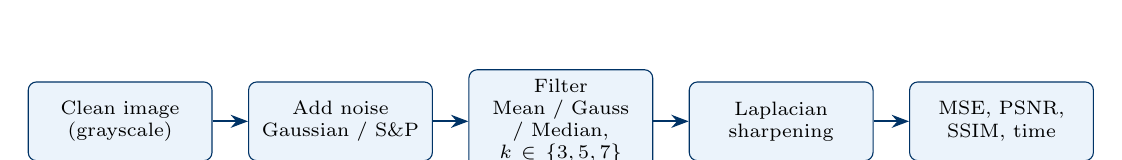
\begin{tikzpicture}[node distance=0.45cm]
    \node[block] (a) {Clean image\\(grayscale)};
    \node[block, right=of a] (b) {Add noise\\Gaussian / S\&P};
    \node[block, right=of b] (c) {Filter\\Mean / Gauss / Median, $k\in\{3,5,7\}$};
    \node[block, right=of c] (d) {Laplacian\\sharpening};
    \node[block, right=of d] (e) {MSE, PSNR, SSIM, time};
    \draw[arrow] (a) -- (b); \draw[arrow] (b) -- (c); \draw[arrow] (c) -- (d); \draw[arrow] (d) -- (e);
\end{tikzpicture}}
\caption{Part A workflow.}
\end{figure}

\subsection{Implementation and Results}
The filters use \texttt{cv2.blur}, \texttt{cv2.GaussianBlur}, \texttt{cv2.medianBlur} and
\texttt{cv2.Laplacian}; metrics use \texttt{skimage.metrics}. Figures~\ref{fig:grid_gauss} and
\ref{fig:grid_sp} show the original, the noisy input and all 12 filter outputs per noise type.
The noisy inputs score 20.61\,dB / SSIM 0.469 (Gaussian) and 15.83\,dB / SSIM 0.390 (S\&P).

\begin{figure}[H]
    \centering
    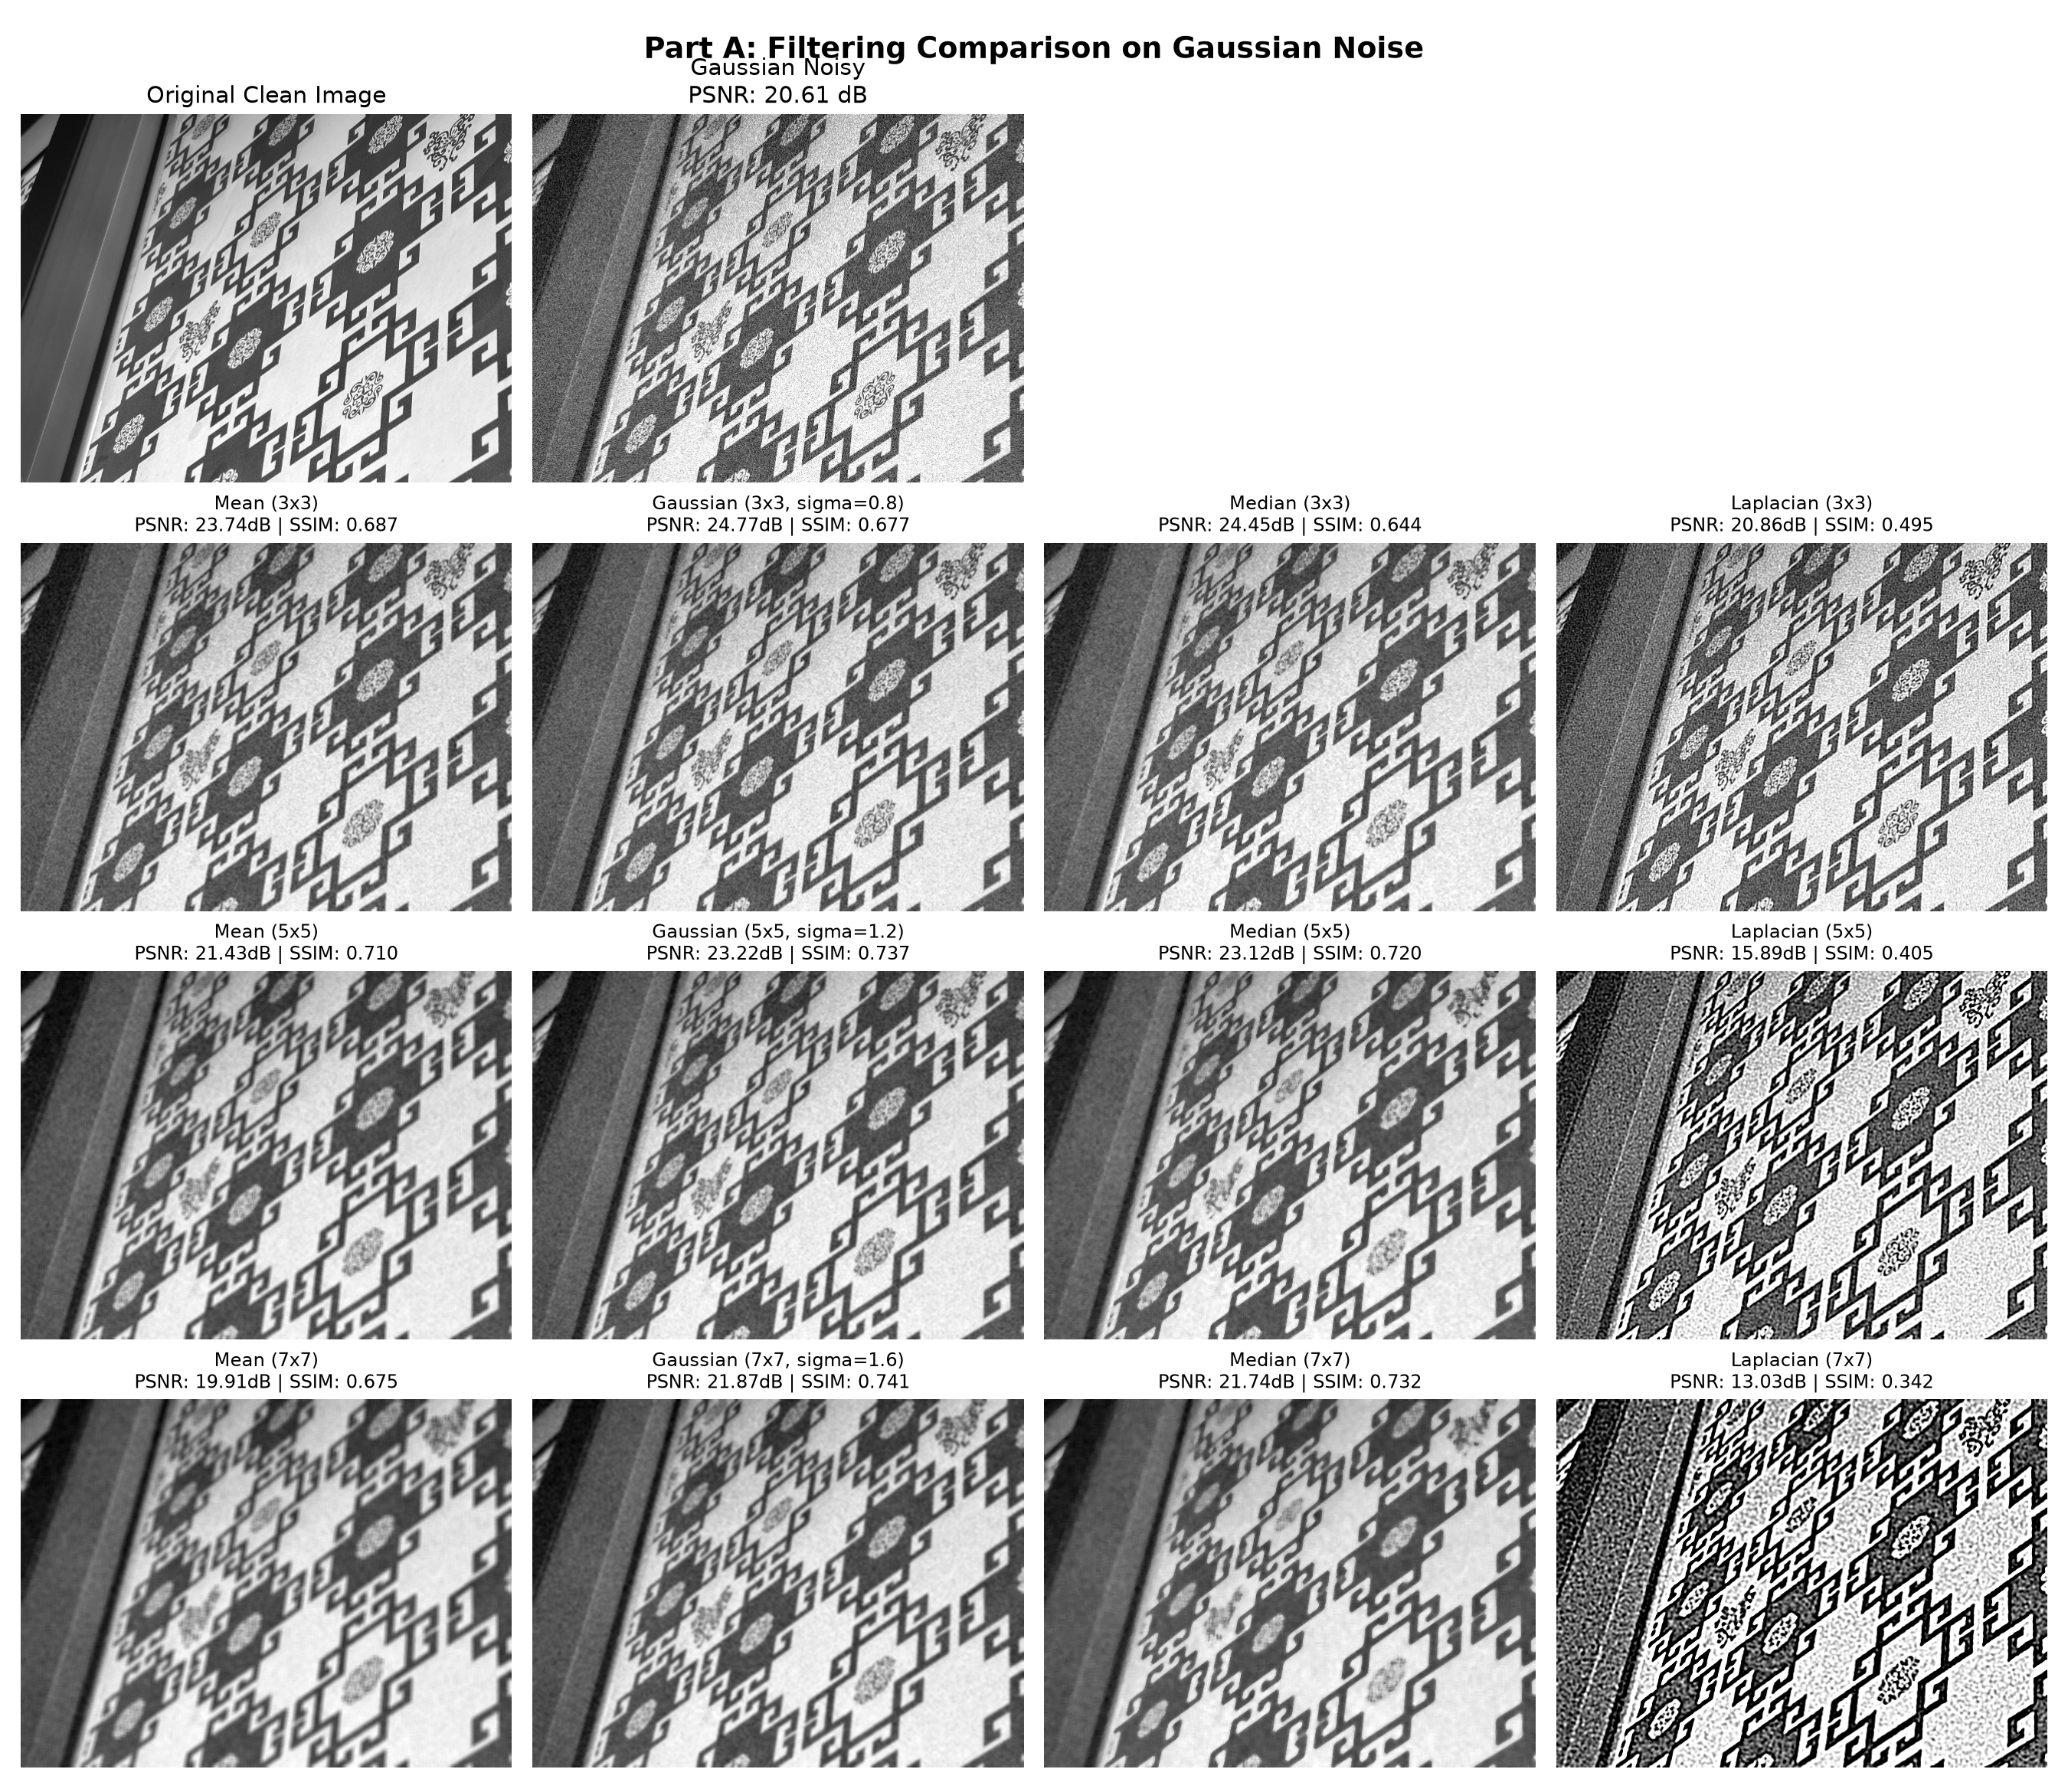
\includegraphics[width=0.92\linewidth]{figures/grid_Gaussian.png}
    \caption{Filtering results on Gaussian noise ($\sigma_n=25$). Rows: kernel $3\times3$, $5\times5$, $7\times7$.}
    \label{fig:grid_gauss}
\end{figure}

\begin{figure}[H]
    \centering
    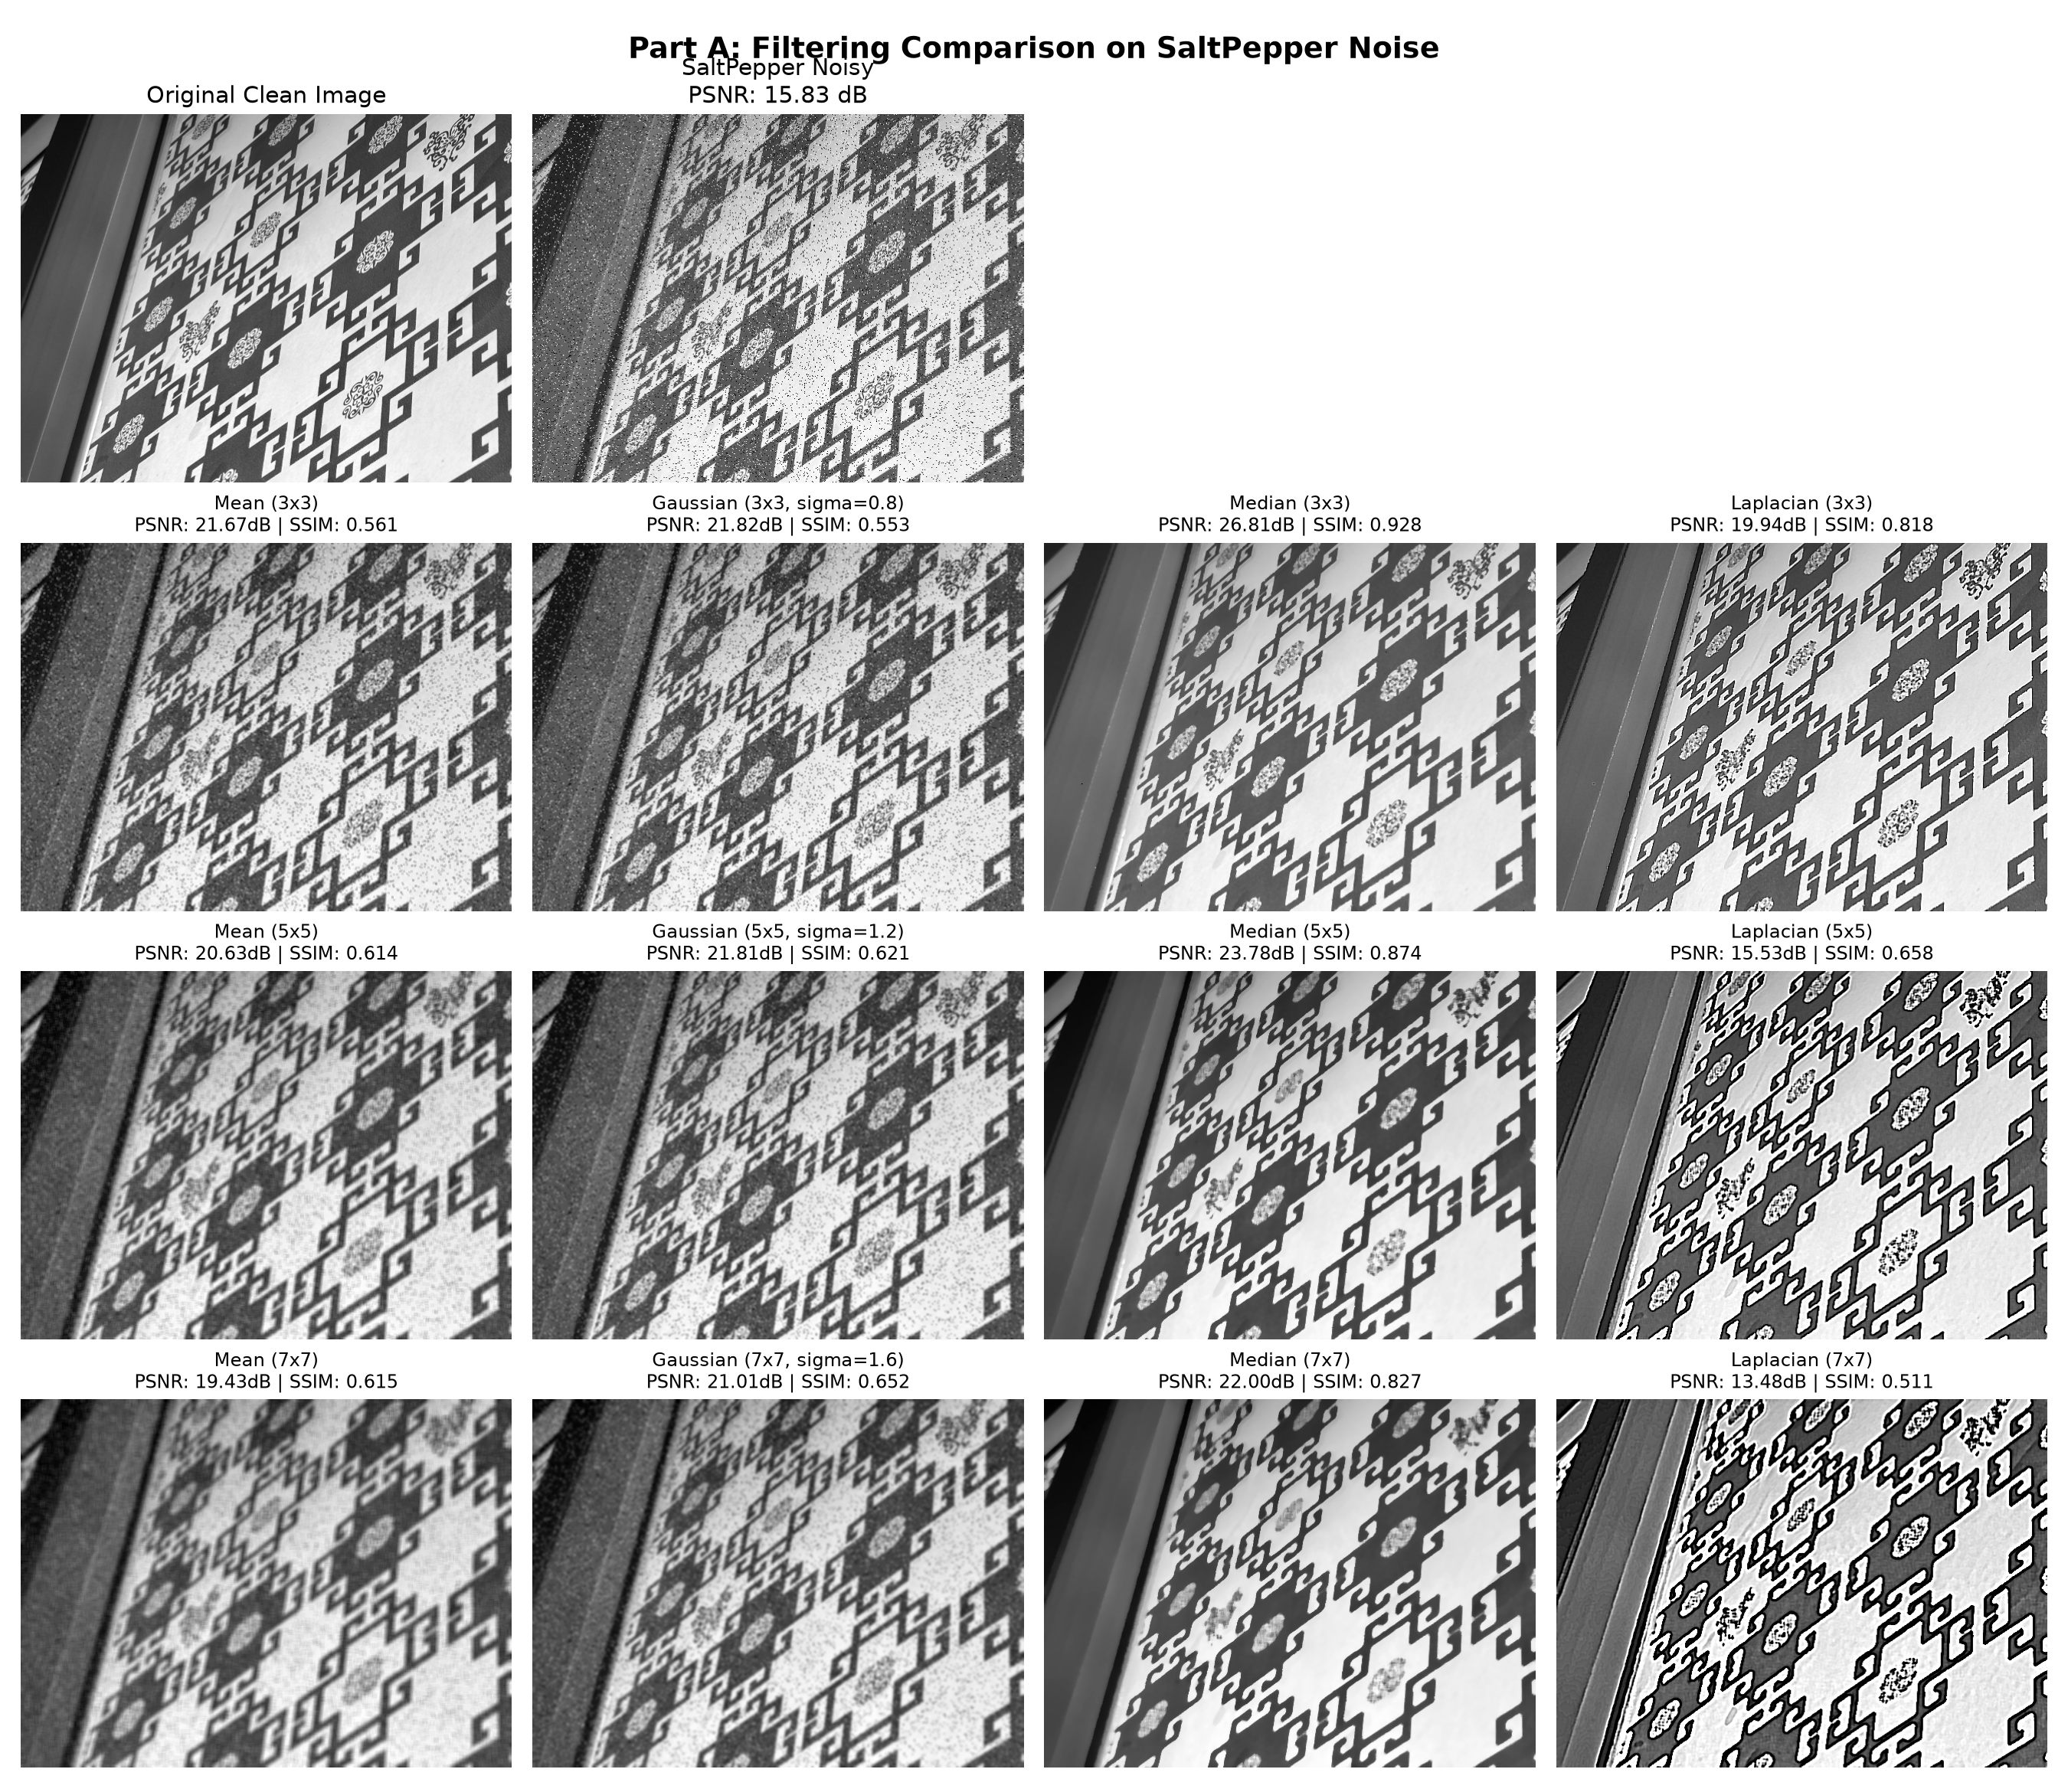
\includegraphics[width=0.92\linewidth]{figures/grid_SaltPepper.png}
    \caption{Filtering results on salt-and-pepper noise (8\%).}
    \label{fig:grid_sp}
\end{figure}

\subsection{Comparative Analysis}

\begin{table}[H]
\centering
\caption{Quantitative comparison of spatial filters (best PSNR per noise type in bold).}
\label{tab:parta}
\resizebox{\linewidth}{!}{\begin{tabular}{llcrrrr}
\toprule
Noise & Filter & Kernel & MSE $\downarrow$ & PSNR (dB) $\uparrow$ & SSIM $\uparrow$ & Time (ms) $\downarrow$ \\
\midrule
Gaussian ($\sigma_n$=25) & Mean & 3$\times$3 & 275.13 & 23.74 & 0.6870 & 1.389 \\
\textbf{Gaussian ($\sigma_n$=25)} & \textbf{Gaussian ($\sigma$=0.8)} & \textbf{3$\times$3} & \textbf{216.71} & \textbf{24.77} & \textbf{0.6768} & \textbf{1.163} \\
Gaussian ($\sigma_n$=25) & Median & 3$\times$3 & 233.37 & 24.45 & 0.6439 & 0.439 \\
Gaussian ($\sigma_n$=25) & Laplacian & 3$\times$3 & 533.73 & 20.86 & 0.4946 & 1.949 \\
\midrule
Gaussian ($\sigma_n$=25) & Mean & 5$\times$5 & 468.23 & 21.43 & 0.7102 & 0.092 \\
Gaussian ($\sigma_n$=25) & Gaussian ($\sigma$=1.2) & 5$\times$5 & 309.70 & 23.22 & 0.7370 & 0.352 \\
Gaussian ($\sigma_n$=25) & Median & 5$\times$5 & 316.77 & 23.12 & 0.7198 & 0.157 \\
Gaussian ($\sigma_n$=25) & Laplacian & 5$\times$5 & 1675.13 & 15.89 & 0.4055 & 2.810 \\
\midrule
Gaussian ($\sigma_n$=25) & Mean & 7$\times$7 & 663.66 & 19.91 & 0.6748 & 0.234 \\
Gaussian ($\sigma_n$=25) & Gaussian ($\sigma$=1.6) & 7$\times$7 & 423.12 & 21.87 & 0.7408 & 0.371 \\
Gaussian ($\sigma_n$=25) & Median & 7$\times$7 & 436.06 & 21.74 & 0.7321 & 0.509 \\
Gaussian ($\sigma_n$=25) & Laplacian & 7$\times$7 & 3237.72 & 13.03 & 0.3421 & 1.848 \\
\midrule
S\&P (8\%) & Mean & 3$\times$3 & 443.03 & 21.67 & 0.5606 & 0.138 \\
S\&P (8\%) & Gaussian ($\sigma$=0.8) & 3$\times$3 & 427.20 & 21.82 & 0.5530 & 0.187 \\
\textbf{S\&P (8\%)} & \textbf{Median} & \textbf{3$\times$3} & \textbf{135.57} & \textbf{26.81} & \textbf{0.9284} & \textbf{0.105} \\
S\&P (8\%) & Laplacian & 3$\times$3 & 659.73 & 19.94 & 0.8179 & 2.021 \\
\midrule
S\&P (8\%) & Mean & 5$\times$5 & 562.61 & 20.63 & 0.6138 & 0.146 \\
S\&P (8\%) & Gaussian ($\sigma$=1.2) & 5$\times$5 & 428.76 & 21.81 & 0.6208 & 0.237 \\
S\&P (8\%) & Median & 5$\times$5 & 272.33 & 23.78 & 0.8740 & 0.205 \\
S\&P (8\%) & Laplacian & 5$\times$5 & 1818.02 & 15.53 & 0.6582 & 1.987 \\
\midrule
S\&P (8\%) & Mean & 7$\times$7 & 741.87 & 19.43 & 0.6154 & 0.371 \\
S\&P (8\%) & Gaussian ($\sigma$=1.6) & 7$\times$7 & 515.76 & 21.01 & 0.6523 & 0.300 \\
S\&P (8\%) & Median & 7$\times$7 & 410.55 & 22.00 & 0.8271 & 0.455 \\
S\&P (8\%) & Laplacian & 7$\times$7 & 2920.78 & 13.48 & 0.5108 & 3.335 \\
\bottomrule
\end{tabular}
}
\end{table}

\begin{figure}[H]
    \centering
    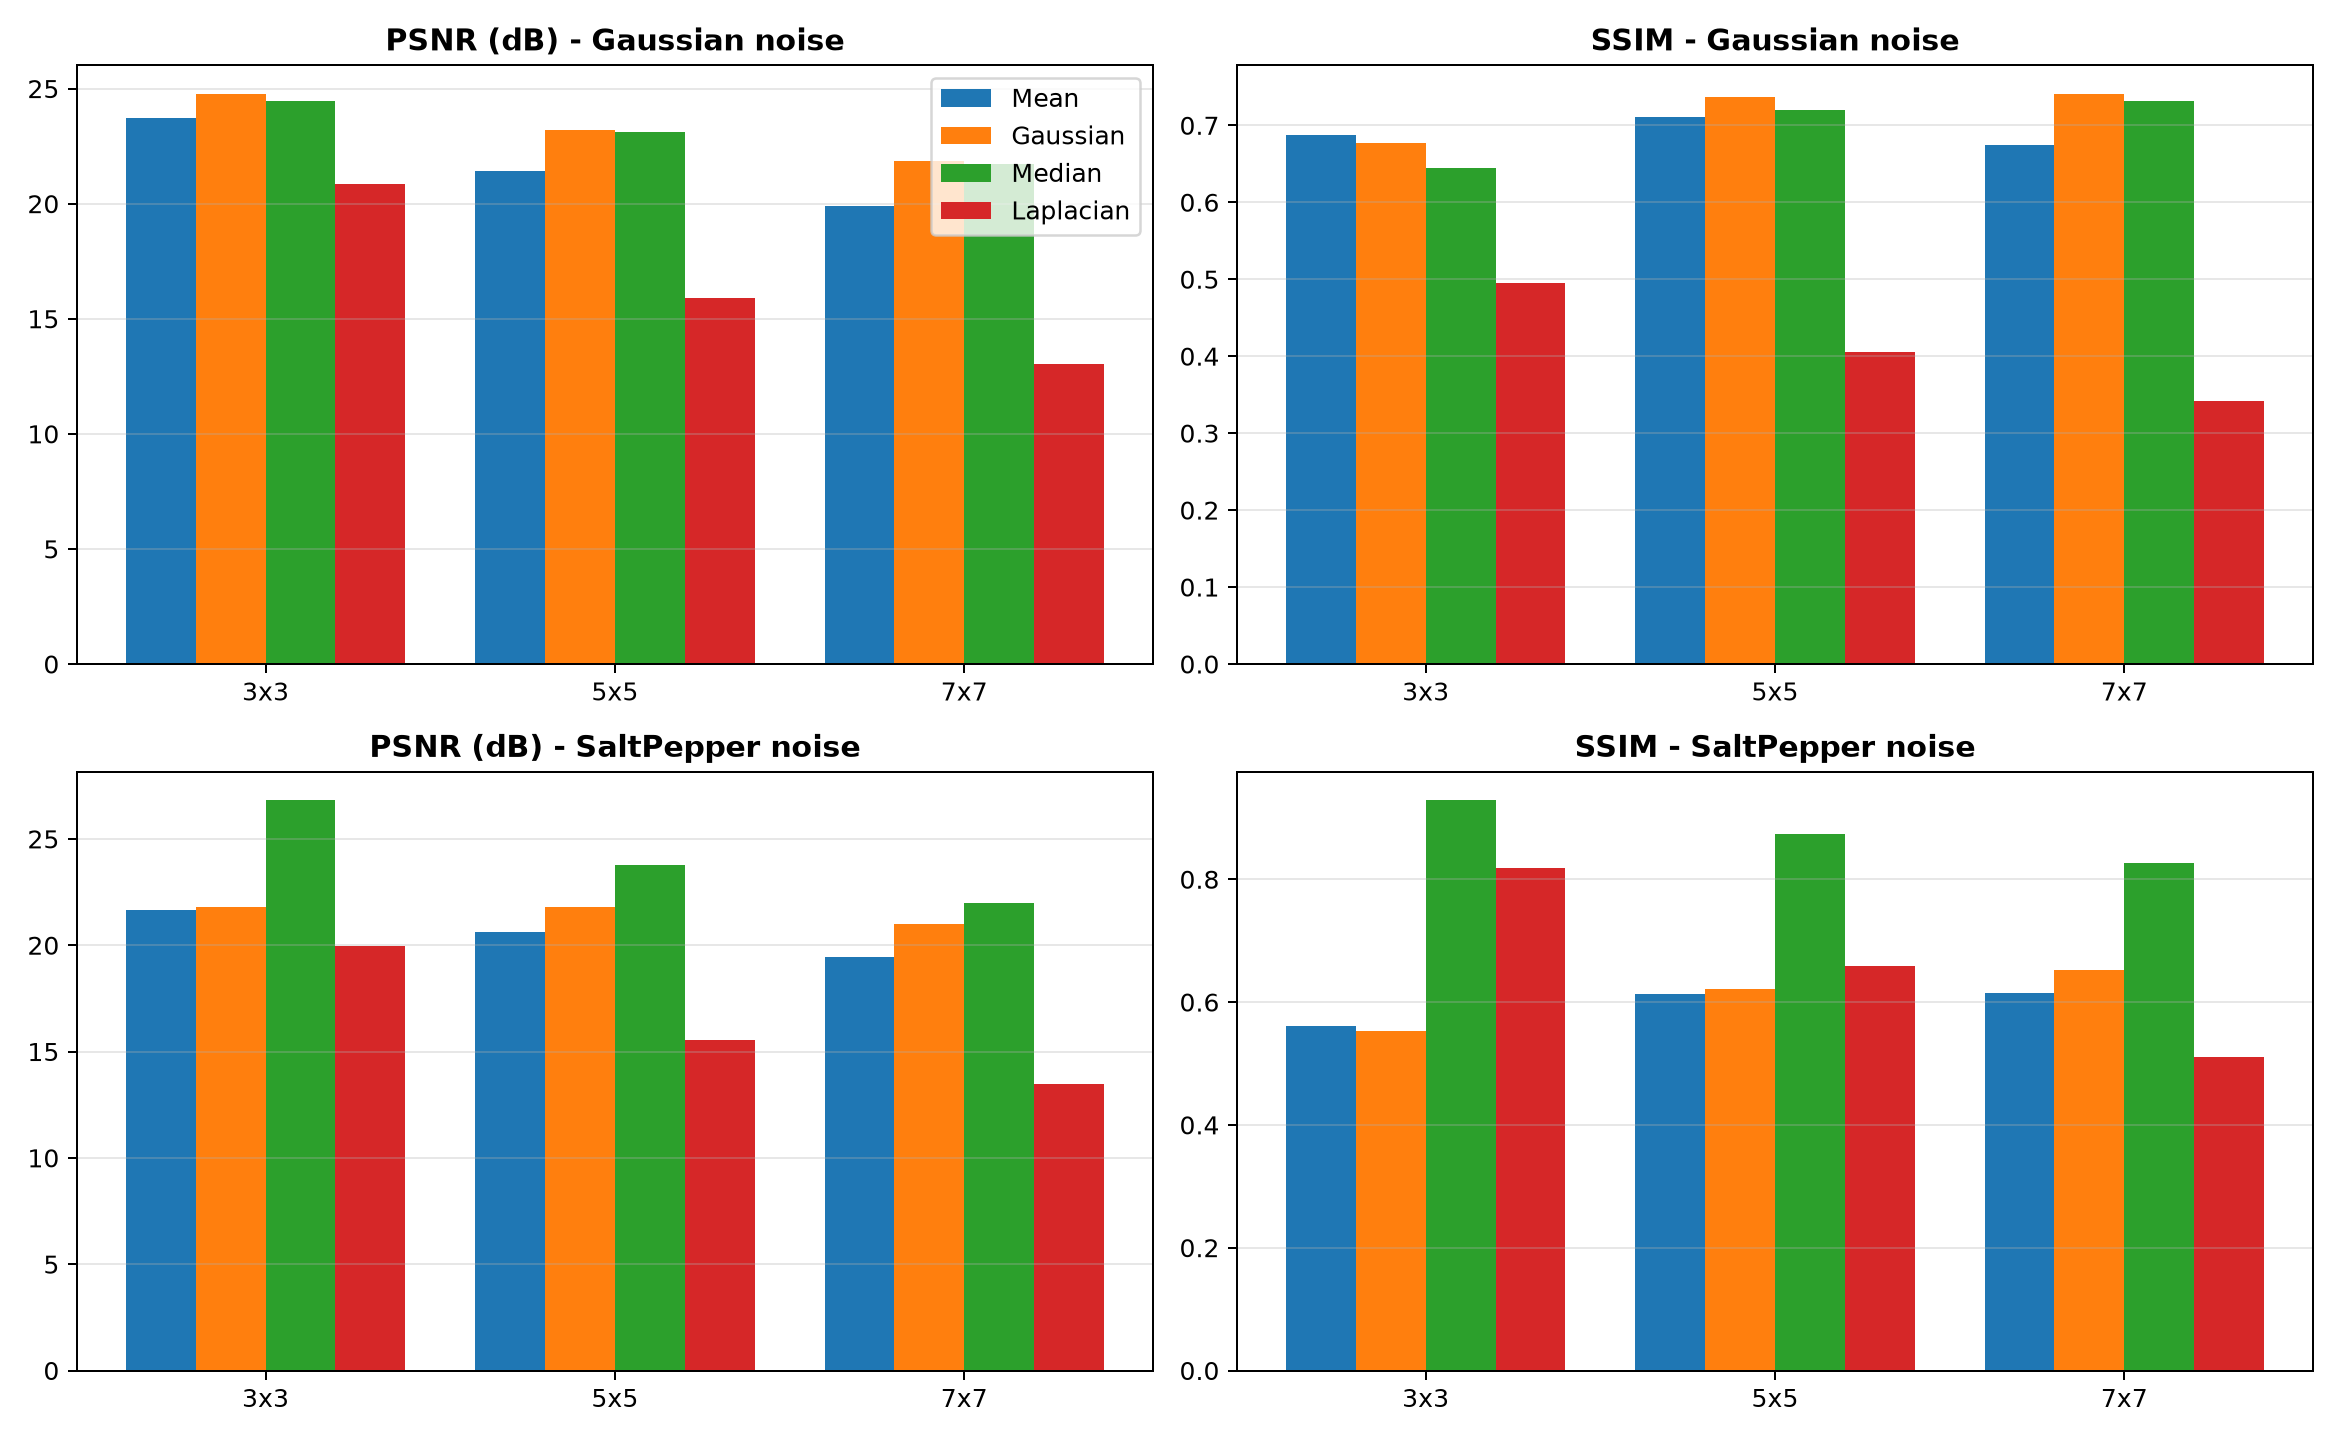
\includegraphics[width=0.9\linewidth]{figures/metrics_bar_chart.png}
    \caption{PSNR and SSIM per filter and kernel size for both noise types.}
    \label{fig:parta_bars}
\end{figure}

\begin{table}[H]
\centering
\caption{Gaussian filter $\sigma$ sensitivity (best PSNR and best SSIM per noise type in bold).}
\label{tab:sigma}
\small
\begin{tabular}{lccrrrr}
\toprule
Noise & $\sigma$ & Kernel & MSE & PSNR (dB) & SSIM & Time (ms) \\
\midrule
\textbf{Gaussian} & \textbf{0.5} & \textbf{5$\times$5} & \textbf{271.73} & \textbf{23.79} & \textbf{0.5636} & \textbf{0.250} \\
Gaussian & 1.0 & 7$\times$7 & 272.76 & 23.77 & 0.7269 & 0.489 \\
\textbf{Gaussian} & \textbf{1.5} & \textbf{11$\times$11} & \textbf{415.00} & \textbf{21.95} & \textbf{0.7420} & \textbf{0.594} \\
Gaussian & 2.0 & 13$\times$13 & 568.51 & 20.58 & 0.7159 & 0.730 \\
Gaussian & 2.5 & 17$\times$17 & 727.07 & 19.52 & 0.6756 & 0.875 \\
Gaussian & 3.0 & 19$\times$19 & 879.84 & 18.69 & 0.6363 & 1.224 \\
\midrule
S\&P & 0.5 & 5$\times$5 & 770.51 & 19.26 & 0.4692 & 0.532 \\
\textbf{S\&P} & \textbf{1.0} & \textbf{7$\times$7} & \textbf{410.13} & \textbf{22.00} & \textbf{0.6039} & \textbf{0.563} \\
S\&P & 1.5 & 11$\times$11 & 509.63 & 21.06 & 0.6515 & 0.774 \\
\textbf{S\&P} & \textbf{2.0} & \textbf{13$\times$13} & \textbf{650.67} & \textbf{20.00} & \textbf{0.6579} & \textbf{0.878} \\
S\&P & 2.5 & 17$\times$17 & 803.27 & 19.08 & 0.6397 & 0.785 \\
S\&P & 3.0 & 19$\times$19 & 952.60 & 18.34 & 0.6133 & 0.902 \\
\bottomrule
\end{tabular}

\end{table}

\begin{figure}[H]
    \centering
    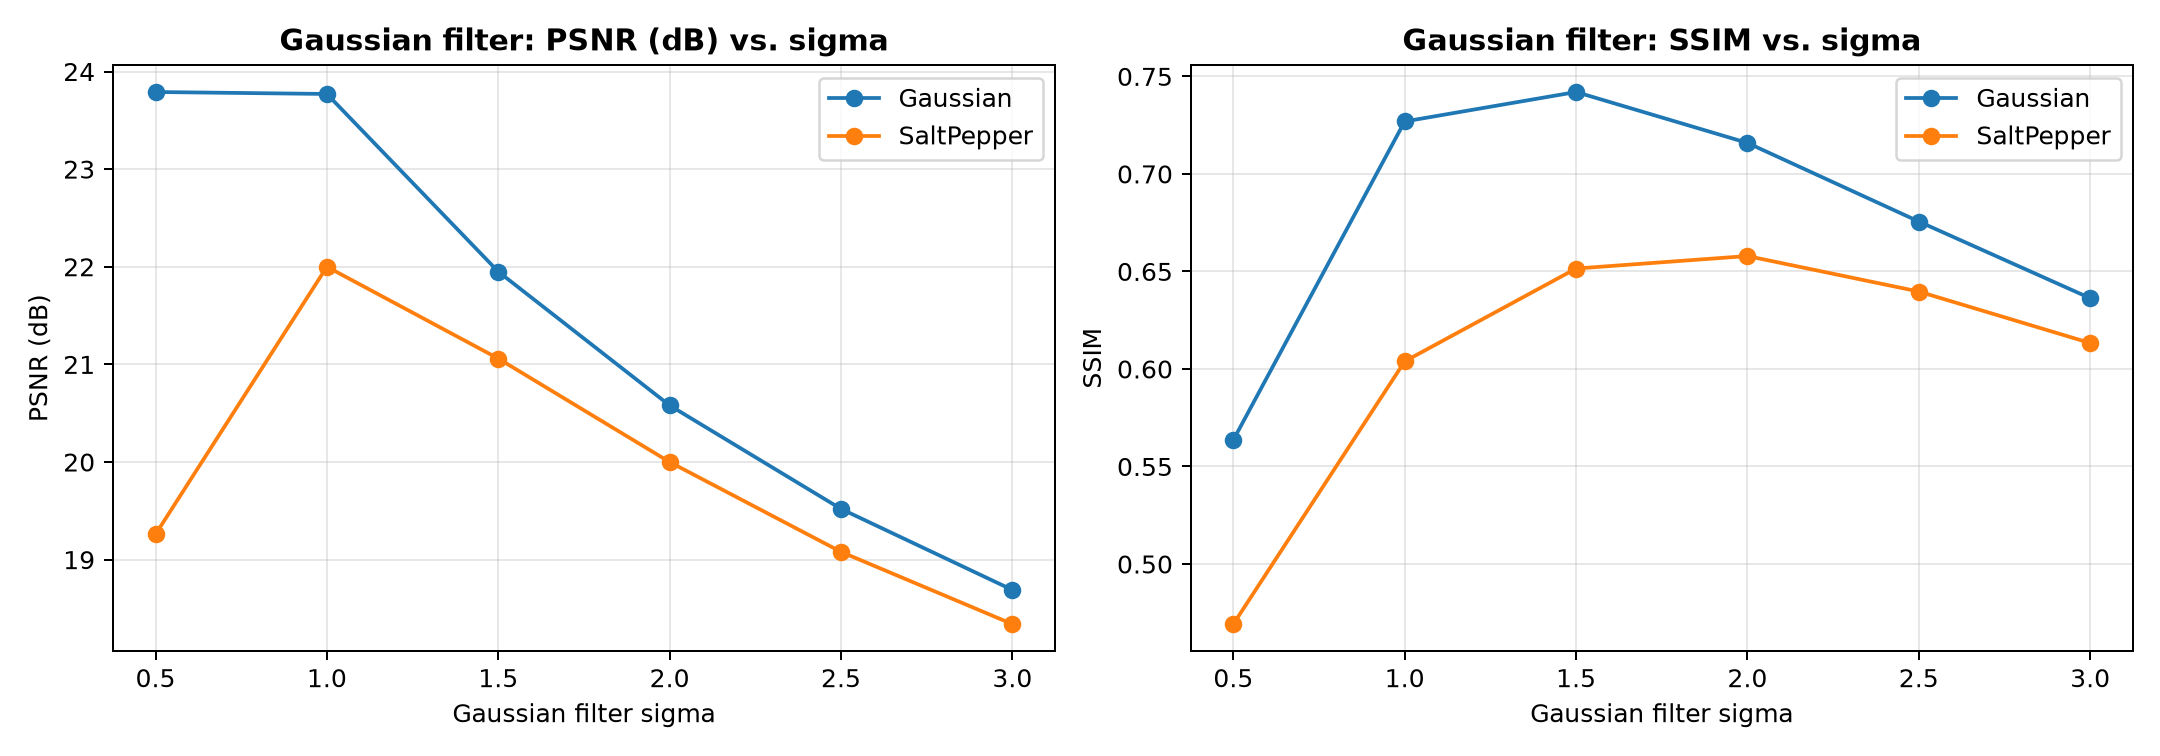
\includegraphics[width=0.85\linewidth]{figures/sigma_sensitivity.png}
    \caption{PSNR and SSIM as a function of the Gaussian filter standard deviation.}
    \label{fig:sigma}
\end{figure}

\textbf{Quantitative analysis.}
\begin{itemize}[leftmargin=*]
    \item \textbf{Salt-and-pepper noise:} the $3\times3$ median filter is the clear winner
          (26.81\,dB, SSIM 0.928), about 5\,dB above the best linear filter. Mean and Gaussian
          filters only spread each impulse over the kernel, so their SSIM stays at 0.55--0.65 for
          every kernel size and every $\sigma$ (Table~\ref{tab:sigma}).
    \item \textbf{Gaussian noise:} PSNR is highest for small kernels (Gaussian $3\times3$, 24.77\,dB;
          median $3\times3$, 24.45\,dB), whereas SSIM peaks with moderate smoothing (Gaussian
          $7\times7$, 0.741; $\sigma=1.5$, 0.742). Stronger smoothing removes more noise, which helps
          local structure, but also blurs the fine ornaments, which costs pixel-wise error.
    \item \textbf{Kernel size:} for every filter, PSNR decreases monotonically from $3\times3$ to
          $7\times7$. The mean filter degrades fastest (23.74 $\rightarrow$ 19.91\,dB) because its
          flat weights blur most; the Gaussian filter degrades slowest.
    \item \textbf{$\sigma$ sweep:} beyond $\sigma\approx1.5$ both PSNR and SSIM drop steadily for both
          noise types, so large $\sigma$ is never beneficial on this detailed image.
    \item \textbf{Runtime:} the denoising filters take only 0.1--0.5\,ms on a $640\times480$ image (the
          very first call, $\approx$1.4\,ms, includes OpenCV warm-up), and the optimized median filter
          is as fast as the linear ones. Laplacian sharpening is the slowest step (1.8--3.3\,ms)
          because it runs in 32-bit floating point and must be converted back to 8-bit.
\end{itemize}

\textbf{Qualitative analysis.}
\begin{itemize}[leftmargin=*]
    \item \textbf{Noise removal vs.\ edge preservation:} the median filter keeps the step edges of the
          geometric pattern sharp, while mean and Gaussian filters produce soft, blurred edges at
          $7\times7$ (over-smoothing). On Gaussian noise, however, the median filter leaves a
          blotchy, ``painted'' texture in flat plaster regions.
    \item \textbf{Linear filters on impulses:} with S\&P noise, mean and Gaussian filters turn each
          impulse into a grey blob that is still clearly visible, which explains their low SSIM.
    \item \textbf{Laplacian sharpening:} at $3\times3$ it visibly crisps edges of the ornaments and
          window frame, but because it is a high-pass operation it also amplifies the residual
          noise and produces thin halo/overshoot bands along strong edges. With larger apertures
          the halos widen and the PSNR falls to 13--16\,dB, even though the image looks sharper.
          Sharpening therefore should only be applied after effective denoising and with a small
          aperture; PSNR/SSIM against the clean image penalise it by design.
\end{itemize}

%=====================================================================
\section{Part B: 3D Reconstruction from Stereo Images}\label{sec:partb}
%=====================================================================
\subsection{Methodology}

\textbf{Epipolar geometry.} Corresponding points $\mathbf x \leftrightarrow \mathbf x'$
(homogeneous) in the left and right images satisfy
\begin{equation}
    \mathbf x'^{\top} F\, \mathbf x = 0, \qquad \mathbf l' = F\mathbf x,\quad \mathbf l = F^{\top}\mathbf x',
\end{equation}
where $F$ is the $3\times3$ rank-2 fundamental matrix and $\mathbf l'$ is the epipolar line of
$\mathbf x$ in the right image. We detect SIFT keypoints, match them with a brute-force KNN
matcher ($k=2$) and Lowe's ratio test (0.75), and estimate $F$ with RANSAC
(\texttt{cv2.findFundamentalMat}, threshold 1.5\,px, confidence 0.99). Two errors are reported over
the RANSAC inliers: the symmetric point-to-epipolar-line distance
$d(\mathbf x,\mathbf l)=|\mathbf l^\top\mathbf x|/\sqrt{l_1^2+l_2^2}$ (averaged over both images) and the
first-order geometric (Sampson) error
\begin{equation}
    e_{S} = \frac{|\mathbf x'^{\top}F\mathbf x|}
    {\sqrt{(F\mathbf x)_1^2+(F\mathbf x)_2^2+(F^{\top}\mathbf x')_1^2+(F^{\top}\mathbf x')_2^2}} .
\end{equation}

\textbf{Dense disparity.} For a rectified pair, a left pixel $(x,y)$ matches $(x-d,y)$ in the
right image.
\begin{itemize}[leftmargin=*]
    \item \textbf{Block Matching (BM)} chooses, independently per pixel, the disparity minimizing the
          sum of absolute differences over a $b\times b$ window:
          $d^*(p)=\arg\min_d\sum_{q\in W_p}|I_L(q)-I_R(q-d)|$.
    \item \textbf{Semi-Global Matching (SGBM)} minimizes a global energy that adds smoothness
          penalties, approximated by dynamic programming along 8 directions (3-way mode):
          \begin{equation}
              E(D)=\sum_p C(p,D_p) + \sum_{q\in N_p} P_1\,[|D_p-D_q|=1] + \sum_{q\in N_p} P_2\,[|D_p-D_q|>1],
          \end{equation}
          with $P_1=8\cdot3\cdot b^2$ and $P_2=32\cdot3\cdot b^2$, uniqueness ratio 10 and speckle filtering.
\end{itemize}

\textbf{Depth and point cloud.} With focal length $f$ and baseline $B$, depth is
$Z = fB/d$. We use \texttt{cv2.reprojectImageTo3D} with
\begin{equation}
    Q=\begin{bmatrix}1&0&0&-c_x\\0&-1&0&c_y\\0&0&0&-f\\0&0&1/B&0\end{bmatrix},\qquad
    [X\;Y\;Z\;W]^\top = Q\,[x\;y\;d\;1]^\top,
\end{equation}
assuming $f=0.8w=512$\,px, $B=0.12$\,m and the principal point at the image centre.

\textbf{Metrics.} Valid disparity ratio (\% of pixels with $d>0$), RMSE and bad-pixel rate
($|d-d_{gt}|>2$\,px) against the ground truth, evaluated on non-occluded pixels with $x\ge128$
(the left band where no full disparity search is possible is excluded identically for all
settings), and runtime.

\begin{figure}[H]
\centering
\resizebox{\linewidth}{!}{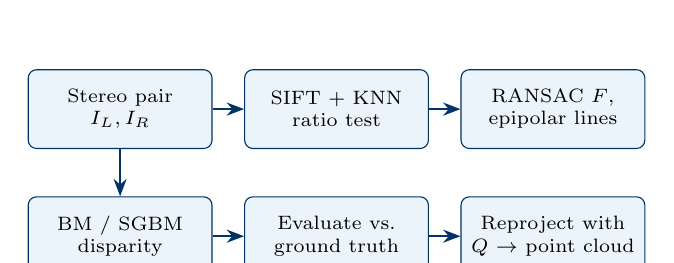
\begin{tikzpicture}[node distance=0.4cm]
    \node[block] (a) {Stereo pair\\$I_L, I_R$};
    \node[block, right=of a] (b) {SIFT + KNN ratio test};
    \node[block, right=of b] (c) {RANSAC $F$, epipolar lines};
    \node[block, below=0.6cm of a] (d) {BM / SGBM disparity};
    \node[block, right=of d] (e) {Evaluate vs.\ ground truth};
    \node[block, right=of e] (f) {Reproject with $Q$ $\rightarrow$ point cloud};
    \draw[arrow] (a) -- (b); \draw[arrow] (b) -- (c);
    \draw[arrow] (a) -- (d); \draw[arrow] (d) -- (e); \draw[arrow] (e) -- (f);
\end{tikzpicture}}
\caption{Part B workflow.}
\end{figure}

\subsection{Implementation and Results}
Figure~\ref{fig:epi} shows 30 inlier correspondences and their epipolar lines. As expected for a
rectified pair, the lines are almost horizontal and each point lies on the line of its partner.
Figure~\ref{fig:disp} compares the ground truth with five BM/SGBM settings, and
Figure~\ref{fig:cloud} shows the reconstructed point cloud (68\,223 coloured points, depth
1.39--3.43\,m, exported to \texttt{results/part\_b/reconstructed\_cloud.ply}).

\begin{figure}[H]
    \centering
    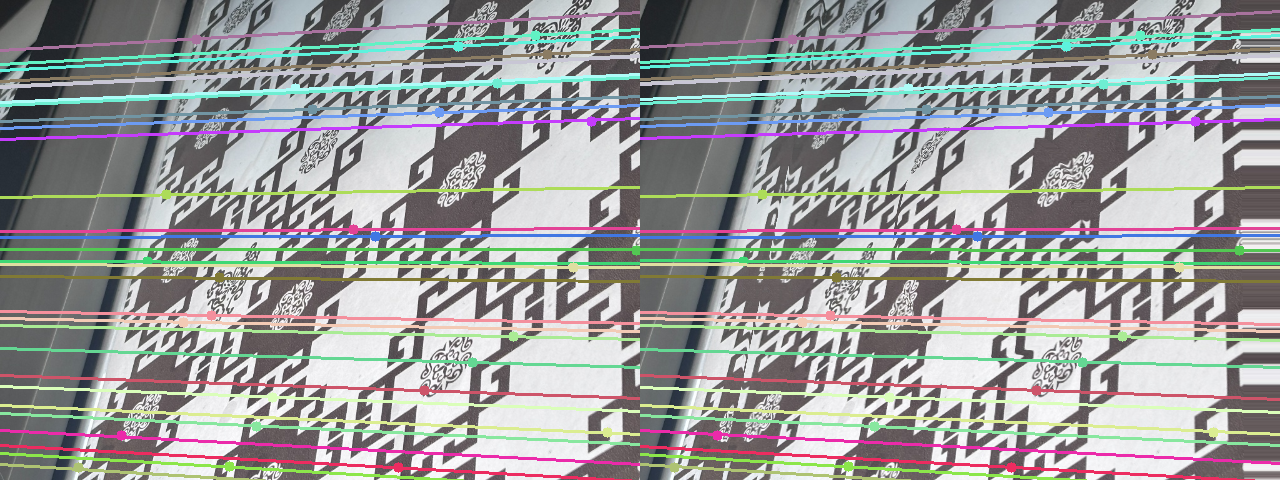
\includegraphics[width=0.95\linewidth]{figures/epipolar_lines.png}
    \caption{Epipolar lines and RANSAC inlier points on the left (left half) and right (right half) images.}
    \label{fig:epi}
\end{figure}

\begin{table}[H]
\centering
\caption{Fundamental matrix estimation (SIFT + RANSAC).}
\label{tab:fund}
\resizebox{\linewidth}{!}{\begin{tabular}{rrrrr}
\toprule
Ratio-test matches & RANSAC inliers & Inlier ratio (\%) & Epipolar err. (px) & Sampson err. (px) \\
\midrule
1277 & 1010 & 79.09 & 0.3388 & 0.2395 \\
\bottomrule
\end{tabular}
}
\end{table}

\begin{figure}[H]
    \centering
    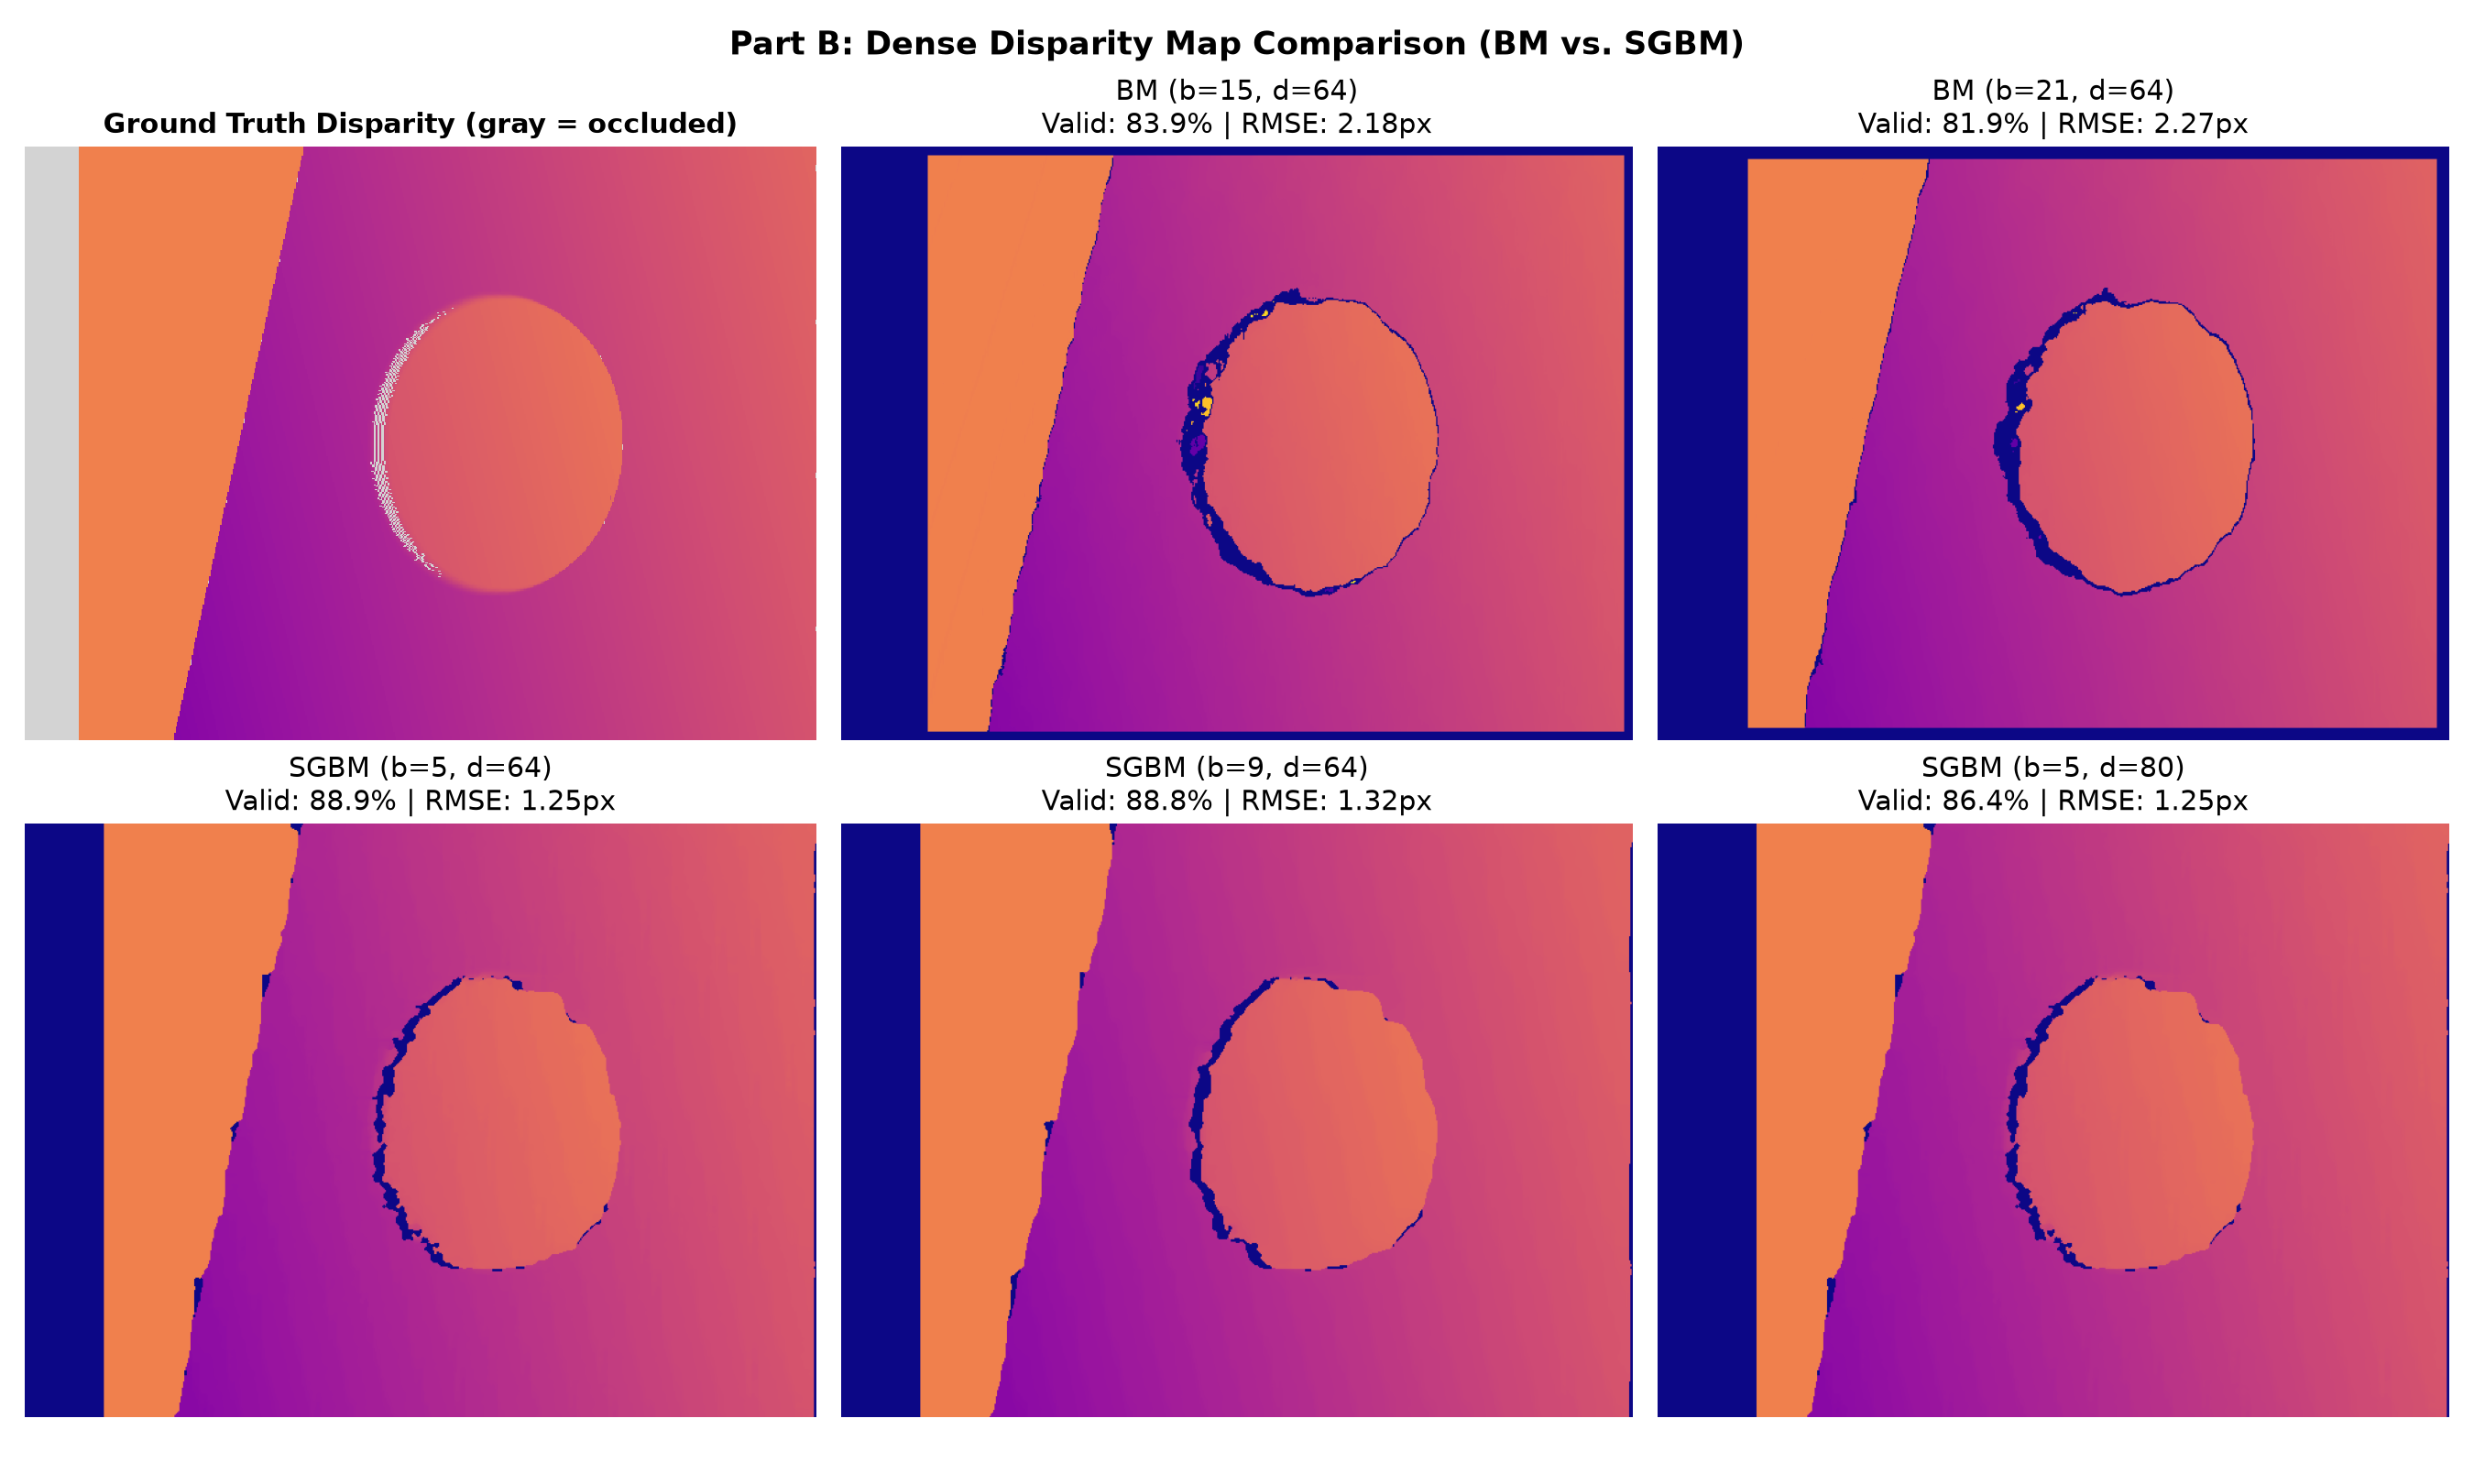
\includegraphics[width=0.95\linewidth]{figures/disparity_comparison.png}
    \caption{Ground truth and colourized disparity maps for BM and SGBM ($b$ = blockSize, $d$ = numDisparities). Dark blue = invalid.}
    \label{fig:disp}
\end{figure}

\begin{figure}[H]
    \centering
    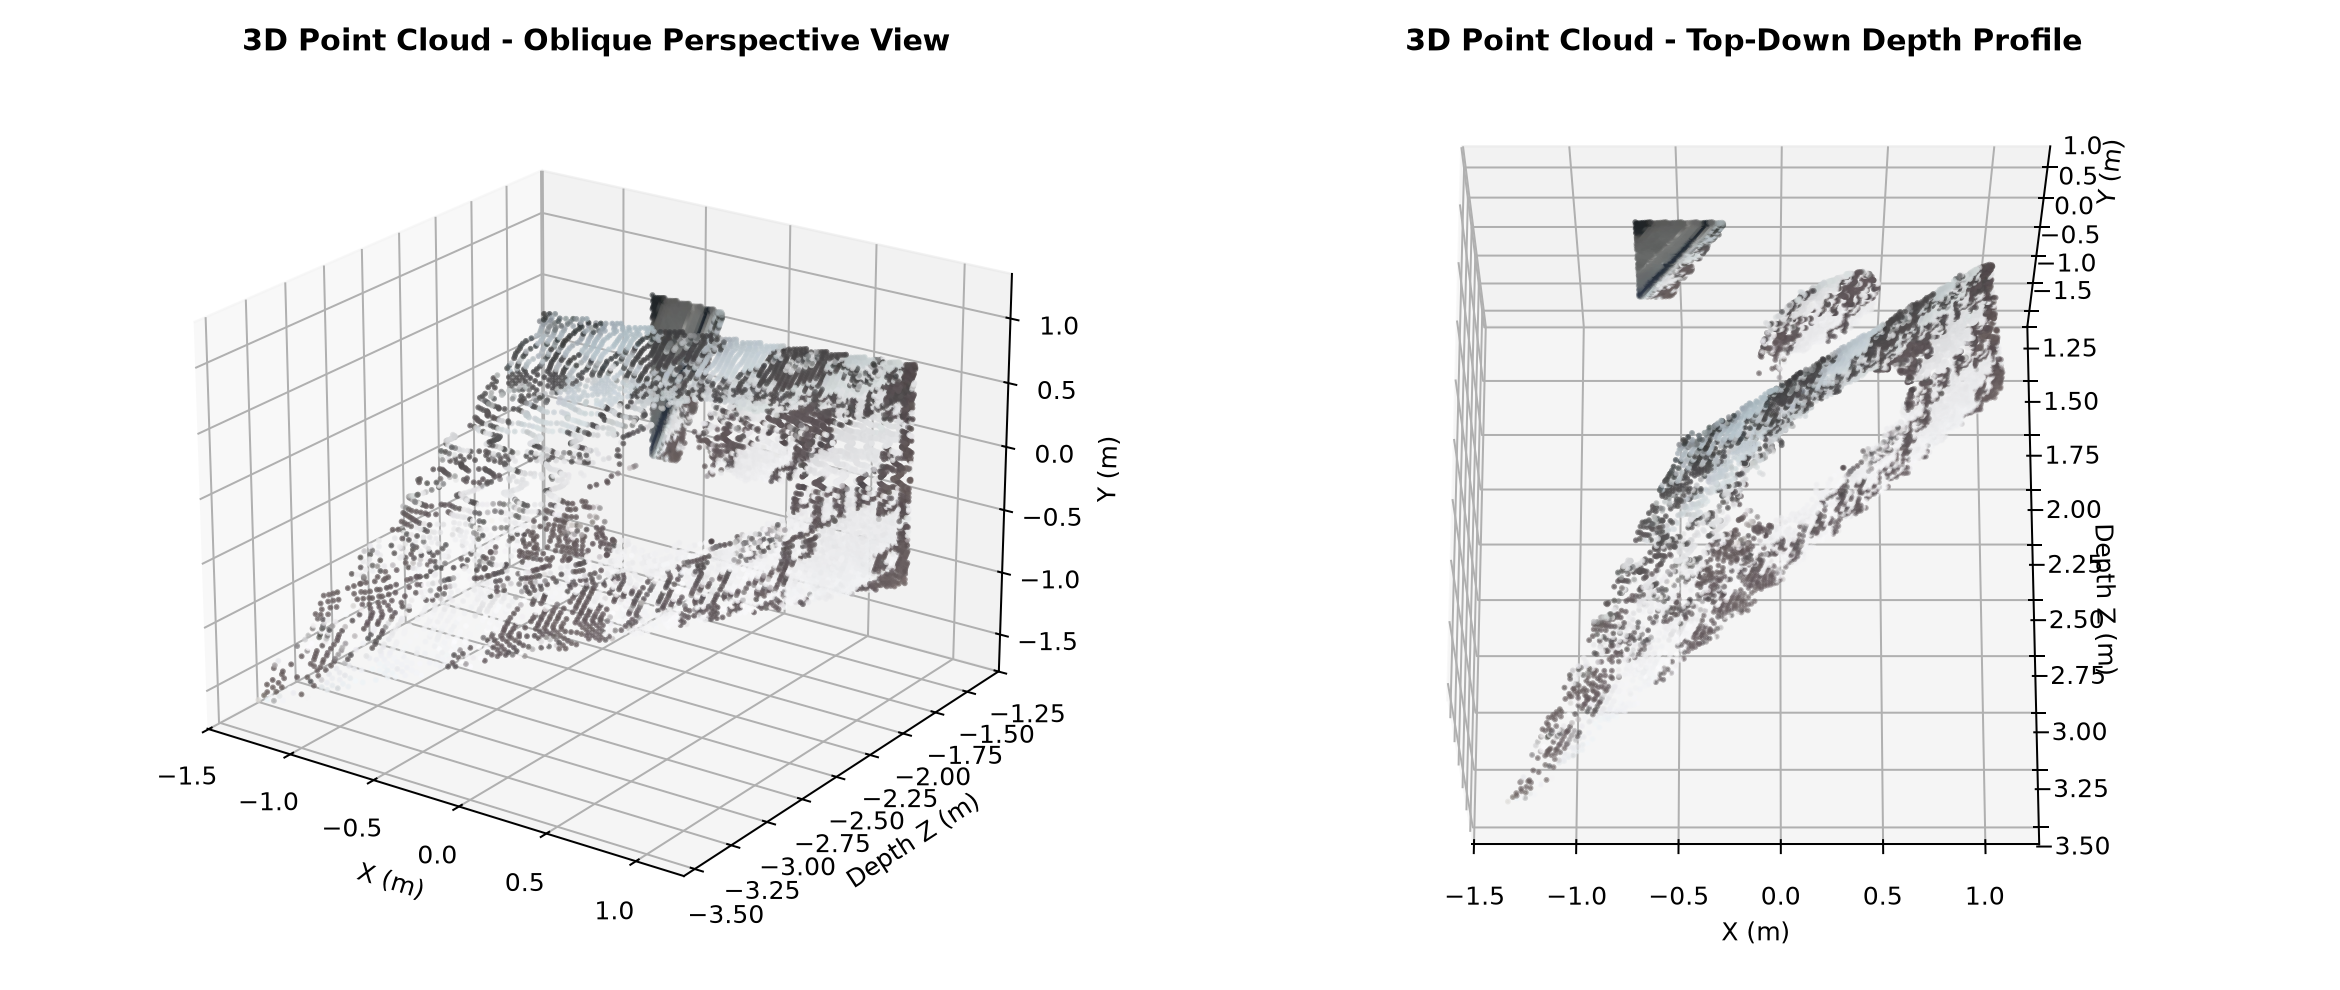
\includegraphics[width=0.95\linewidth]{figures/point_cloud_views.png}
    \caption{Two views of the 3D point cloud reconstructed from SGBM ($b=9$, $d=64$).}
    \label{fig:cloud}
\end{figure}

\subsection{Comparative Analysis}

\begin{table}[H]
\centering
\caption{BM vs.\ SGBM (best RMSE in bold).}
\label{tab:partb}
\resizebox{\linewidth}{!}{\begin{tabular}{lccrrrr}
\toprule
Method & blockSize & numDisp. & Valid (\%) $\uparrow$ & RMSE (px) $\downarrow$ & Bad $>$2px (\%) $\downarrow$ & Runtime (ms) $\downarrow$ \\
\midrule
BM & 15 & 64 & 83.94 & 2.18 & 1.16 & 8.7 \\
BM & 21 & 64 & 81.95 & 2.27 & 1.32 & 8.9 \\
\textbf{SGBM} & \textbf{5} & \textbf{64} & \textbf{88.91} & \textbf{1.25} & \textbf{1.09} & \textbf{19.5} \\
SGBM & 9 & 64 & 88.83 & 1.32 & 1.16 & 23.7 \\
SGBM & 5 & 80 & 86.40 & 1.25 & 1.09 & 26.1 \\
\bottomrule
\end{tabular}
}
\end{table}

\begin{figure}[H]
    \centering
    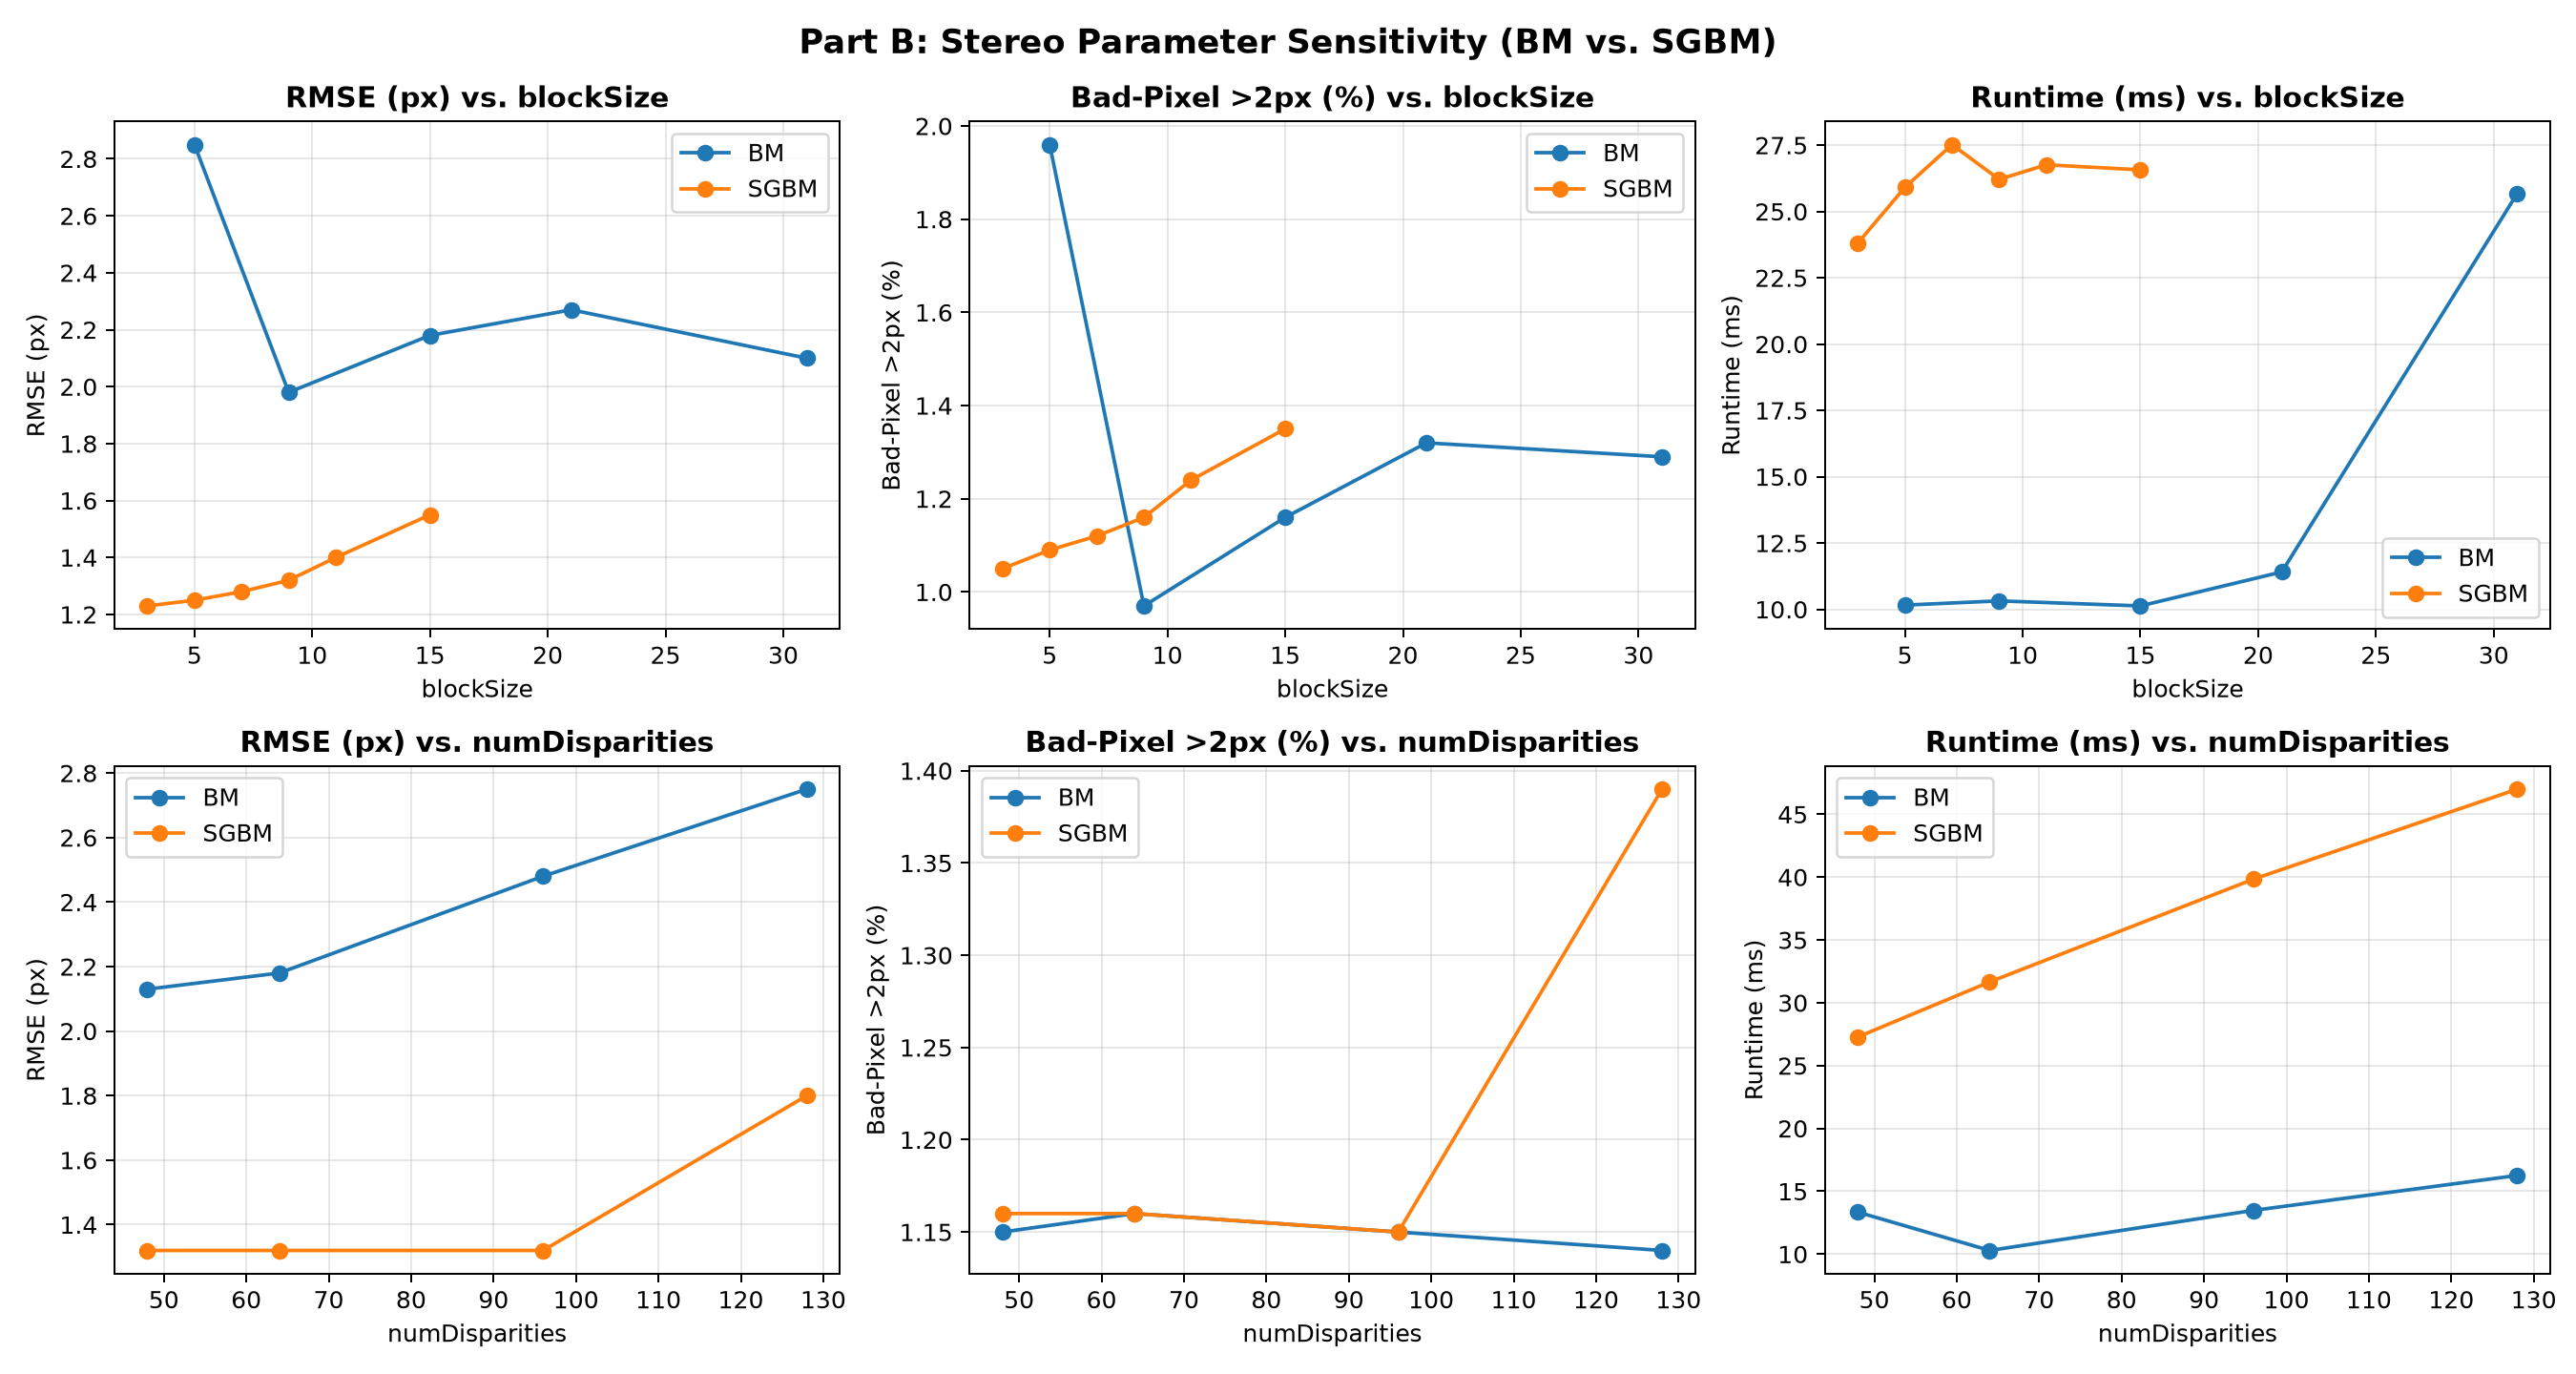
\includegraphics[width=0.95\linewidth]{figures/parameter_sensitivity.png}
    \caption{Sensitivity of BM and SGBM to blockSize (top, numDisparities = 64) and numDisparities (bottom).}
    \label{fig:sens}
\end{figure}

\textbf{Quantitative analysis.}
\begin{itemize}[leftmargin=*]
    \item \textbf{Epipolar geometry:} 79\% of the 1\,277 ratio-test matches survive RANSAC, with a
          mean epipolar distance of 0.34\,px and Sampson error of 0.24\,px, i.e.\ sub-pixel
          consistency, so the estimated $F$ is reliable.
    \item \textbf{BM vs.\ SGBM:} at the same numDisparities, SGBM produces about 5 percentage points
          more valid pixels (88.9\% vs.\ 83.9\%) and roughly 43\% lower RMSE (1.25 vs.\ 2.18\,px).
          The bad-pixel rate is low for both ($\approx$1.1\%), meaning BM's extra error is spread as
          small inaccuracies rather than gross mismatches. SGBM is about 2--3 times slower
          (19.5 vs.\ 8.7\,ms) because it aggregates costs along several paths, and its runtime grows
          linearly with numDisparities (27 $\rightarrow$ 47\,ms from 48 to 128 levels), whereas BM stays
          around 10--16\,ms.
    \item \textbf{blockSize:} BM is unstable with small windows ($b=5$: RMSE 2.85\,px, 1.96\% bad
          pixels) and is best around $b=9$; larger windows lose valid pixels (78.7\% at $b=31$).
          SGBM is much less sensitive thanks to its smoothness term; its error grows slowly from
          1.23\,px ($b=3$) to 1.55\,px ($b=15$) as windows start to straddle depth edges.
    \item \textbf{numDisparities:} the valid ratio falls linearly with numDisparities because
          the leftmost numDisparities columns cannot be matched. Since the maximum ground-truth
          disparity is 44\,px, 48 levels are already sufficient; 128 levels increase ambiguity
          (SGBM RMSE 1.80\,px) and runtime without any benefit.
\end{itemize}

\textbf{Qualitative analysis.}
\begin{itemize}[leftmargin=*]
    \item \textbf{Smoothness:} the wall is densely textured, so both methods recover the slanted
          disparity ramp smoothly; this also explains the low bad-pixel rates. BM additionally
          loses a frame of about half a block width on every image border.
    \item \textbf{Occlusions:} in the occluded strip on the left of the elliptical relief (grey in the
          ground truth) no correspondence exists. BM still assigns disparities there, producing
          blobs of grossly wrong (too large) values, whereas SGBM's uniqueness check mostly marks
          these pixels invalid, which is the desired behaviour.
    \item \textbf{Object boundaries:} BM ``fattens'' the foreground pillar into the background by
          roughly half a window because the SAD window straddles the depth edge. SGBM keeps the
          boundary closer to the ground truth but shows small jagged streaks along it, a typical
          artefact of path-wise cost aggregation.
    \item \textbf{3D geometry:} the point cloud correctly separates the pillar (nearest, $\approx$1.4\,m),
          the raised relief, and the slanted wall receding to $\approx$3.4\,m. Depth quantization
          (disparity steps of 1/16\,px) is visible as slight layering in the top-down view.
\end{itemize}

%=====================================================================
\section{Part C: Multi-View Image Stitching}\label{sec:partc}
%=====================================================================
\subsection{Methodology}

\textbf{Feature extraction.}
\begin{itemize}[leftmargin=*]
    \item \textbf{SIFT:} Difference-of-Gaussian extrema in scale space, sub-pixel refined, with a
          128-D gradient-orientation histogram descriptor (L2 distance).
    \item \textbf{ORB:} oriented FAST corners with rotated BRIEF 256-bit binary descriptors
          (Hamming distance), limited to 3\,000 features per image.
    \item \textbf{AKAZE:} keypoints in a non-linear diffusion scale space, which preserves edges
          better than Gaussian blurring, with binary M-LDB descriptors (Hamming distance).
\end{itemize}

\textbf{Matching.} Brute-force KNN ($k=2$) with Lowe's ratio test: a match $m$ is kept if
$\|f-f_1\| < 0.75\,\|f-f_2\|$, where $f_1,f_2$ are the nearest and second-nearest descriptors.

\textbf{Homography.} For a planar scene or pure camera rotation, corresponding points satisfy
\begin{equation}
    \lambda\begin{bmatrix}x'\\y'\\1\end{bmatrix} = H\begin{bmatrix}x\\y\\1\end{bmatrix},\qquad
    H=\begin{bmatrix}h_{11}&h_{12}&h_{13}\\h_{21}&h_{22}&h_{23}\\h_{31}&h_{32}&h_{33}\end{bmatrix},
\end{equation}
with 8 degrees of freedom, estimated by the DLT inside RANSAC with a reprojection threshold of
2 or 4\,px. Accuracy is measured as the inlier reprojection RMSE
$\sqrt{\frac1N\sum_i\|\mathbf x_i - \pi(H\mathbf x'_i)\|^2}$.

\textbf{Warping.} View 2 is the reference frame. Homographies are chained as
$H_{1\to2}$, $I$, $H_{3\to2}$ and $H_{4\to2}=H_{3\to2}H_{4\to3}$; all images are warped
with an extra translation so that the panorama has non-negative coordinates.

\textbf{Blending.}
\begin{itemize}[leftmargin=*]
    \item \textbf{Feathering:} weights are proportional to the Euclidean distance transform of each
          valid mask, $w_k = D_k/(D_1+D_2)$, so each image fades out towards its border.
    \item \textbf{Laplacian pyramid (multi-band):} each image is decomposed into band-pass levels
          $L_\ell = G_\ell - \mathrm{up}(G_{\ell+1})$, and each level is blended with a Gaussian-blurred
          version of the binary seam mask $M_\ell$:
          $L^{\text{out}}_\ell = (1-M_\ell)L^A_\ell + M_\ell L^B_\ell$, then the pyramid is collapsed. Low
          frequencies (exposure) are mixed over a wide region while high frequencies (edges) switch
          over a narrow one, which avoids both visible seams and ghosting.
    \item \textbf{None (overwrite)} is used as a baseline.
\end{itemize}

\begin{figure}[H]
\centering
\resizebox{\linewidth}{!}{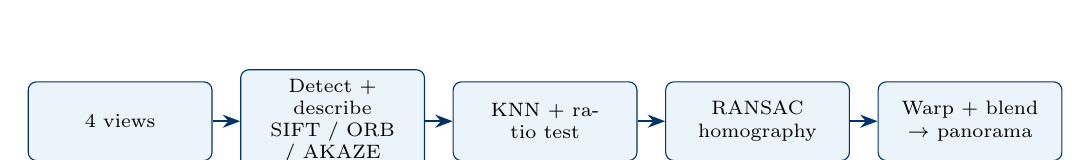
\begin{tikzpicture}[node distance=0.35cm]
    \node[block] (a) {4 views};
    \node[block, right=of a] (b) {Detect + describe\\SIFT / ORB / AKAZE};
    \node[block, right=of b] (c) {KNN + ratio test};
    \node[block, right=of c] (d) {RANSAC homography};
    \node[block, right=of d] (e) {Warp + blend $\rightarrow$ panorama};
    \draw[arrow] (a) -- (b); \draw[arrow] (b) -- (c); \draw[arrow] (c) -- (d); \draw[arrow] (d) -- (e);
\end{tikzpicture}}
\caption{Part C workflow.}
\end{figure}

\subsection{Implementation and Results}
The pipeline is built from the following OpenCV functions:
\begin{itemize}[leftmargin=*, itemsep=0pt]
    \item detection: \texttt{SIFT\_create}, \texttt{ORB\_create}, \texttt{AKAZE\_create};
    \item matching and geometry: \texttt{BFMatcher.knnMatch}, \texttt{findHomography} (RANSAC),
          \texttt{warpPerspective};
    \item blending (with NumPy): \texttt{distanceTransform}, \texttt{pyrDown}, \texttt{pyrUp}.
\end{itemize}
Figure~\ref{fig:views} shows the input views,
Figure~\ref{fig:kps} the detected keypoints, and Figure~\ref{fig:stitch} the inlier matches
between views 2 and 3 with the final panoramas.

\begin{figure}[H]
    \centering
    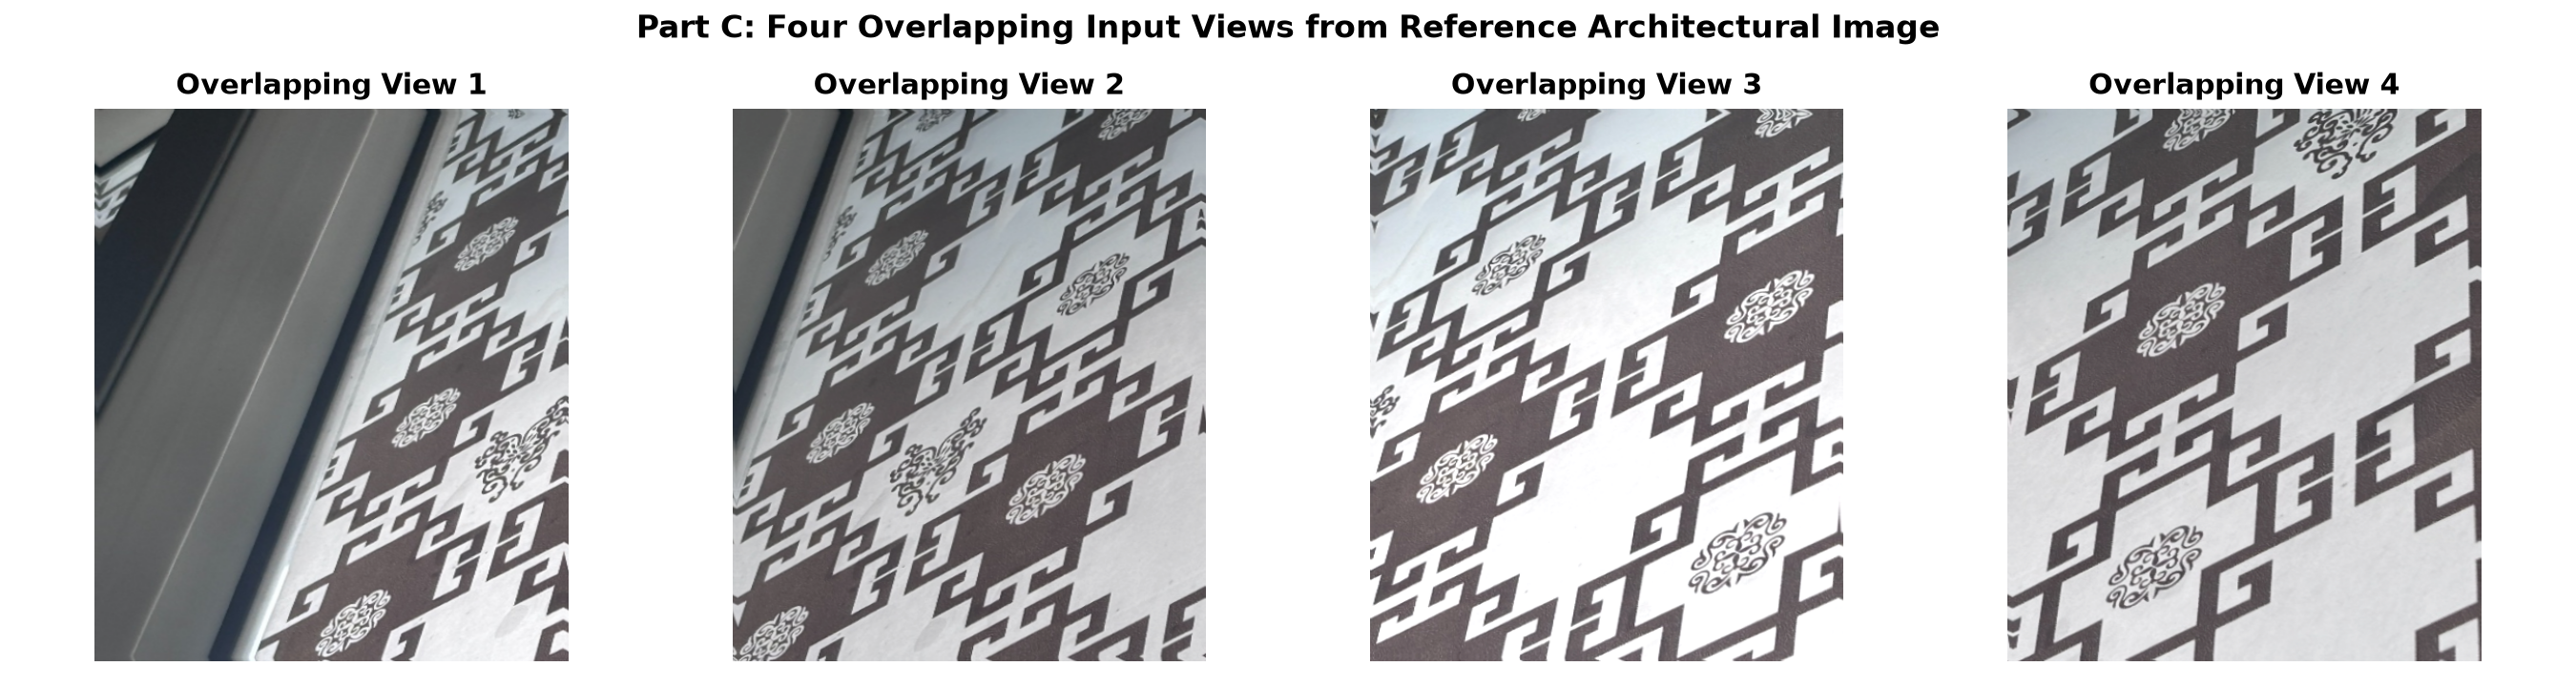
\includegraphics[width=\linewidth]{figures/input_4_views.png}
    \caption{The four overlapping input views (different perspective and exposure).}
    \label{fig:views}
\end{figure}

\begin{figure}[H]
    \centering
    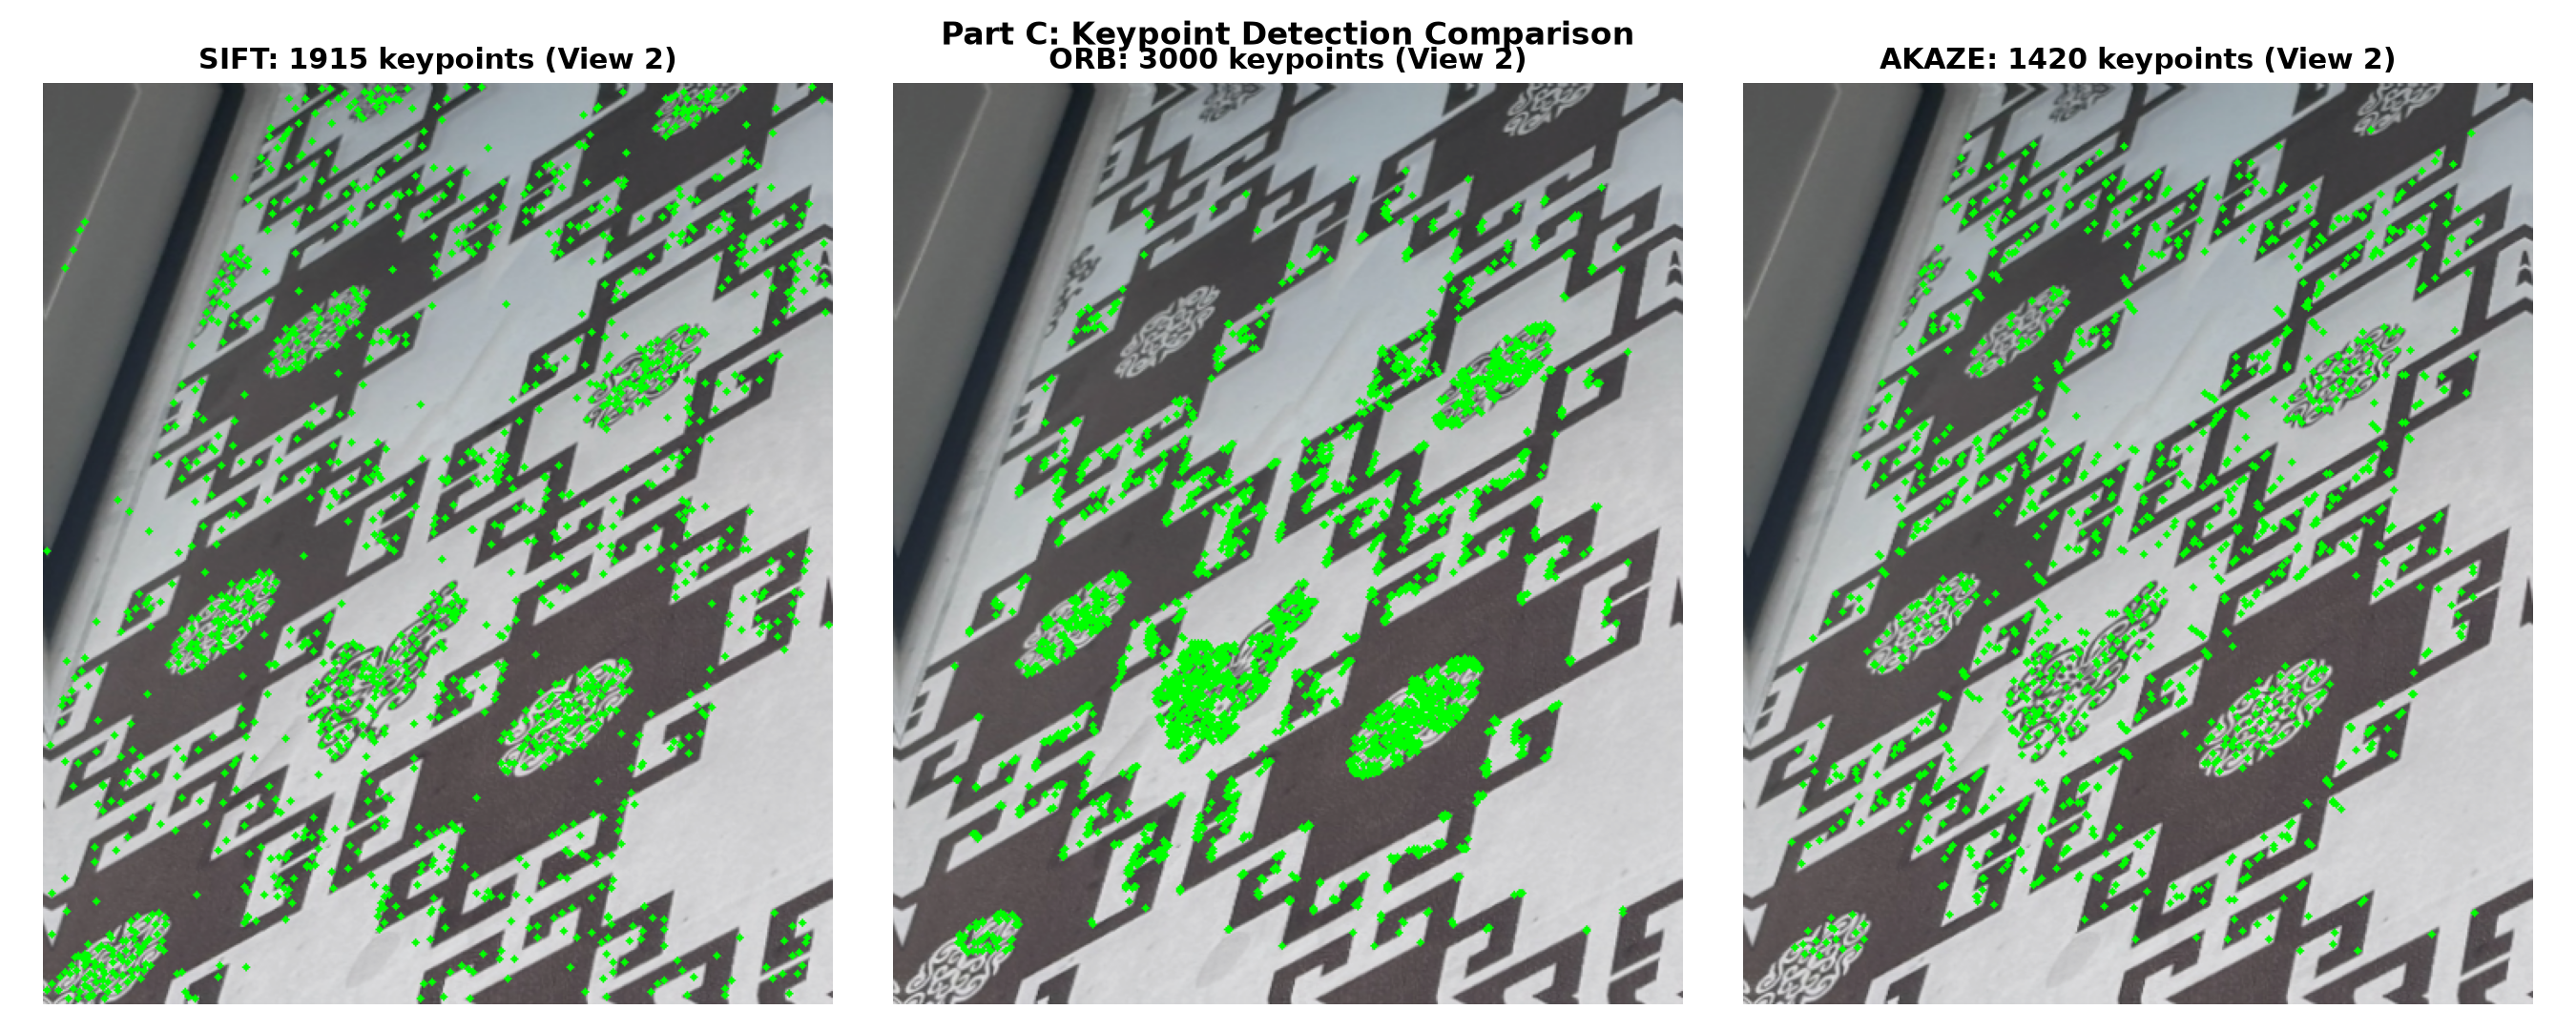
\includegraphics[width=\linewidth]{figures/keypoints_comparison.png}
    \caption{Keypoints detected on view 2 by SIFT, ORB and AKAZE.}
    \label{fig:kps}
\end{figure}

\begin{figure}[H]
    \centering
    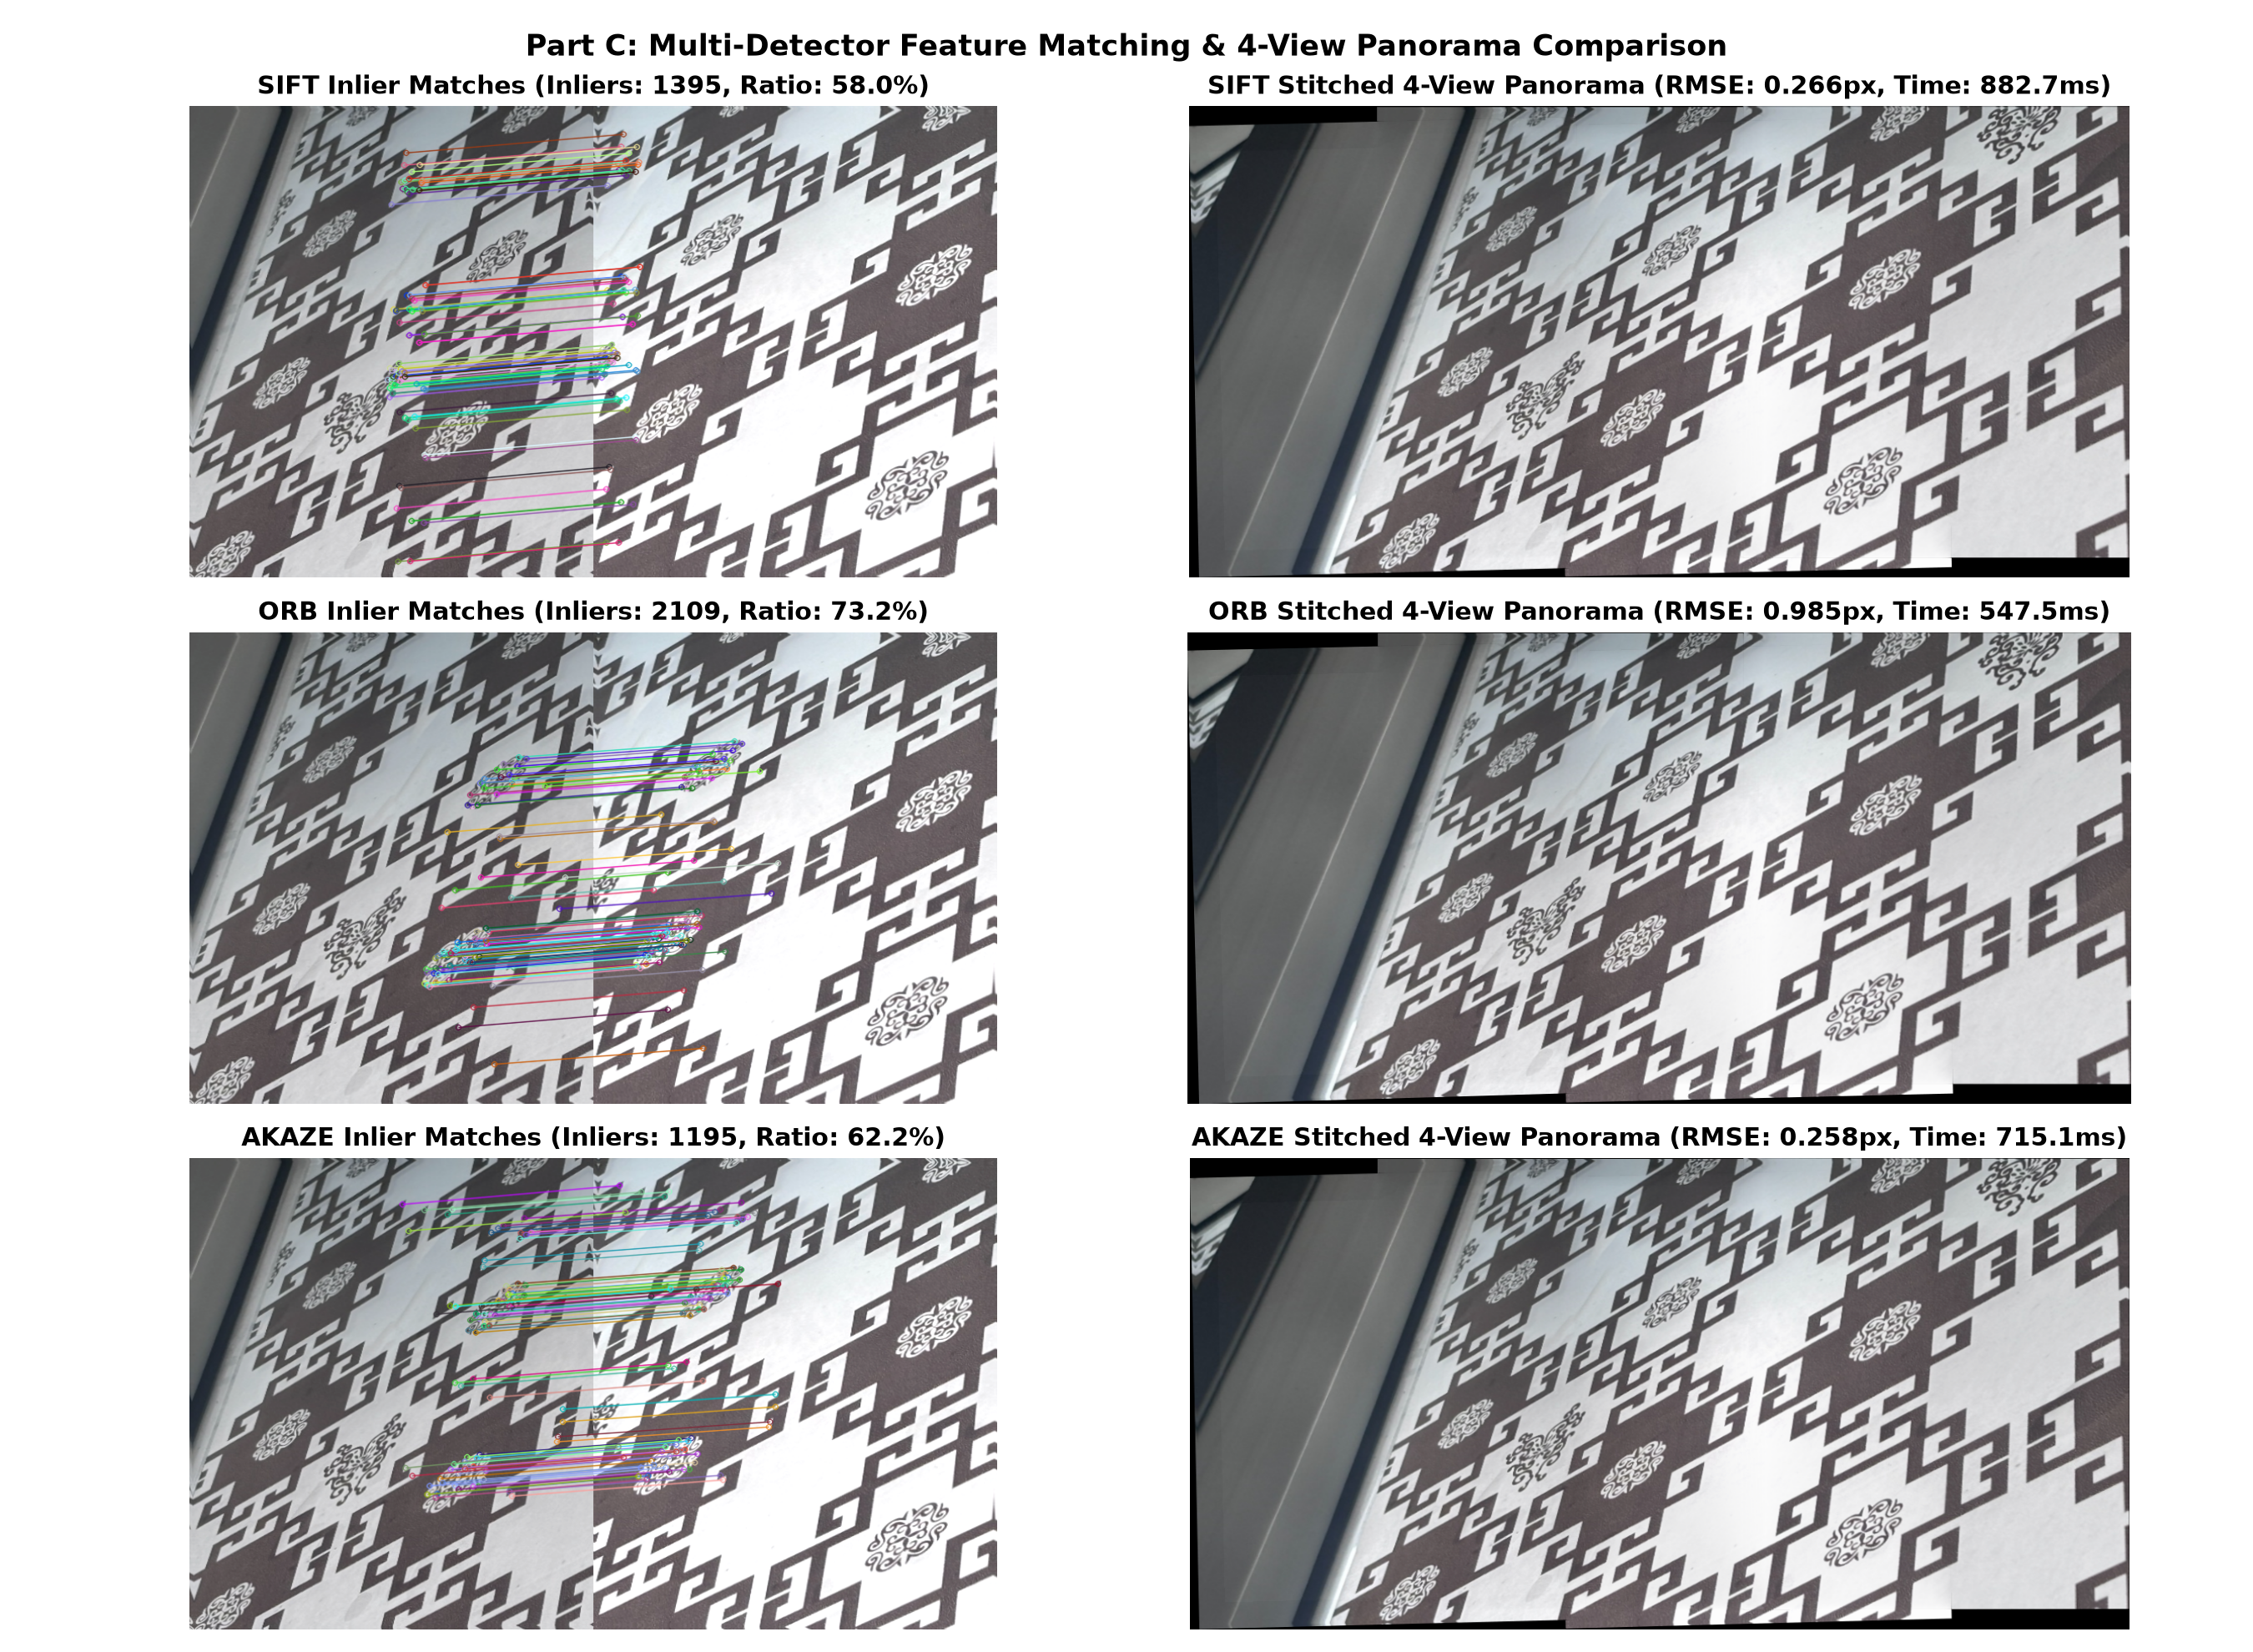
\includegraphics[width=\linewidth]{figures/stitching_comparison.png}
    \caption{RANSAC inlier matches (views 2--3, first 80 shown) and 4-view panoramas (feather blending, RANSAC 4\,px).}
    \label{fig:stitch}
\end{figure}

\subsection{Comparative Analysis}

\begin{table}[H]
\centering
\caption{Detector comparison summed over the three image pairs (best RMSE in bold). Inlier ratio and RMSE are averaged over the pairs.}
\label{tab:partc}
\resizebox{\linewidth}{!}{\begin{tabular}{lcrrrrrr}
\toprule
Detector & RANSAC (px) & Keypoints & Matches & Inliers & Inlier (\%) & RMSE (px) & Time (ms) \\
\midrule
\textbf{SIFT} & \textbf{2.0} & \textbf{9976} & \textbf{2394} & \textbf{1392} & \textbf{57.84} & \textbf{0.232} & \textbf{813.4} \\
SIFT & 4.0 & 9976 & 2394 & 1395 & 57.95 & 0.266 & 882.7 \\
ORB & 2.0 & 17593 & 2873 & 2010 & 69.79 & 0.874 & 781.0 \\
ORB & 4.0 & 17593 & 2873 & 2109 & 73.23 & 0.985 & 547.5 \\
AKAZE & 4.0 & 7167 & 1912 & 1195 & 62.16 & 0.258 & 715.1 \\
\bottomrule
\end{tabular}
}
\end{table}

\begin{table}[H]
\centering
\caption{Blending comparison (SIFT, RANSAC 4\,px).}
\label{tab:blend}
\small
\begin{tabular}{lrr}
\toprule
Blending method & Blending time (ms) & Total time (ms) \\
\midrule
None (overwrite) & 155.8 & 594.3 \\
Feather (distance transform) & 381.6 & 1149.3 \\
Laplacian pyramid (5 levels) & 598.4 & 1286.9 \\
\bottomrule
\end{tabular}

\end{table}

\begin{figure}[H]
    \centering
    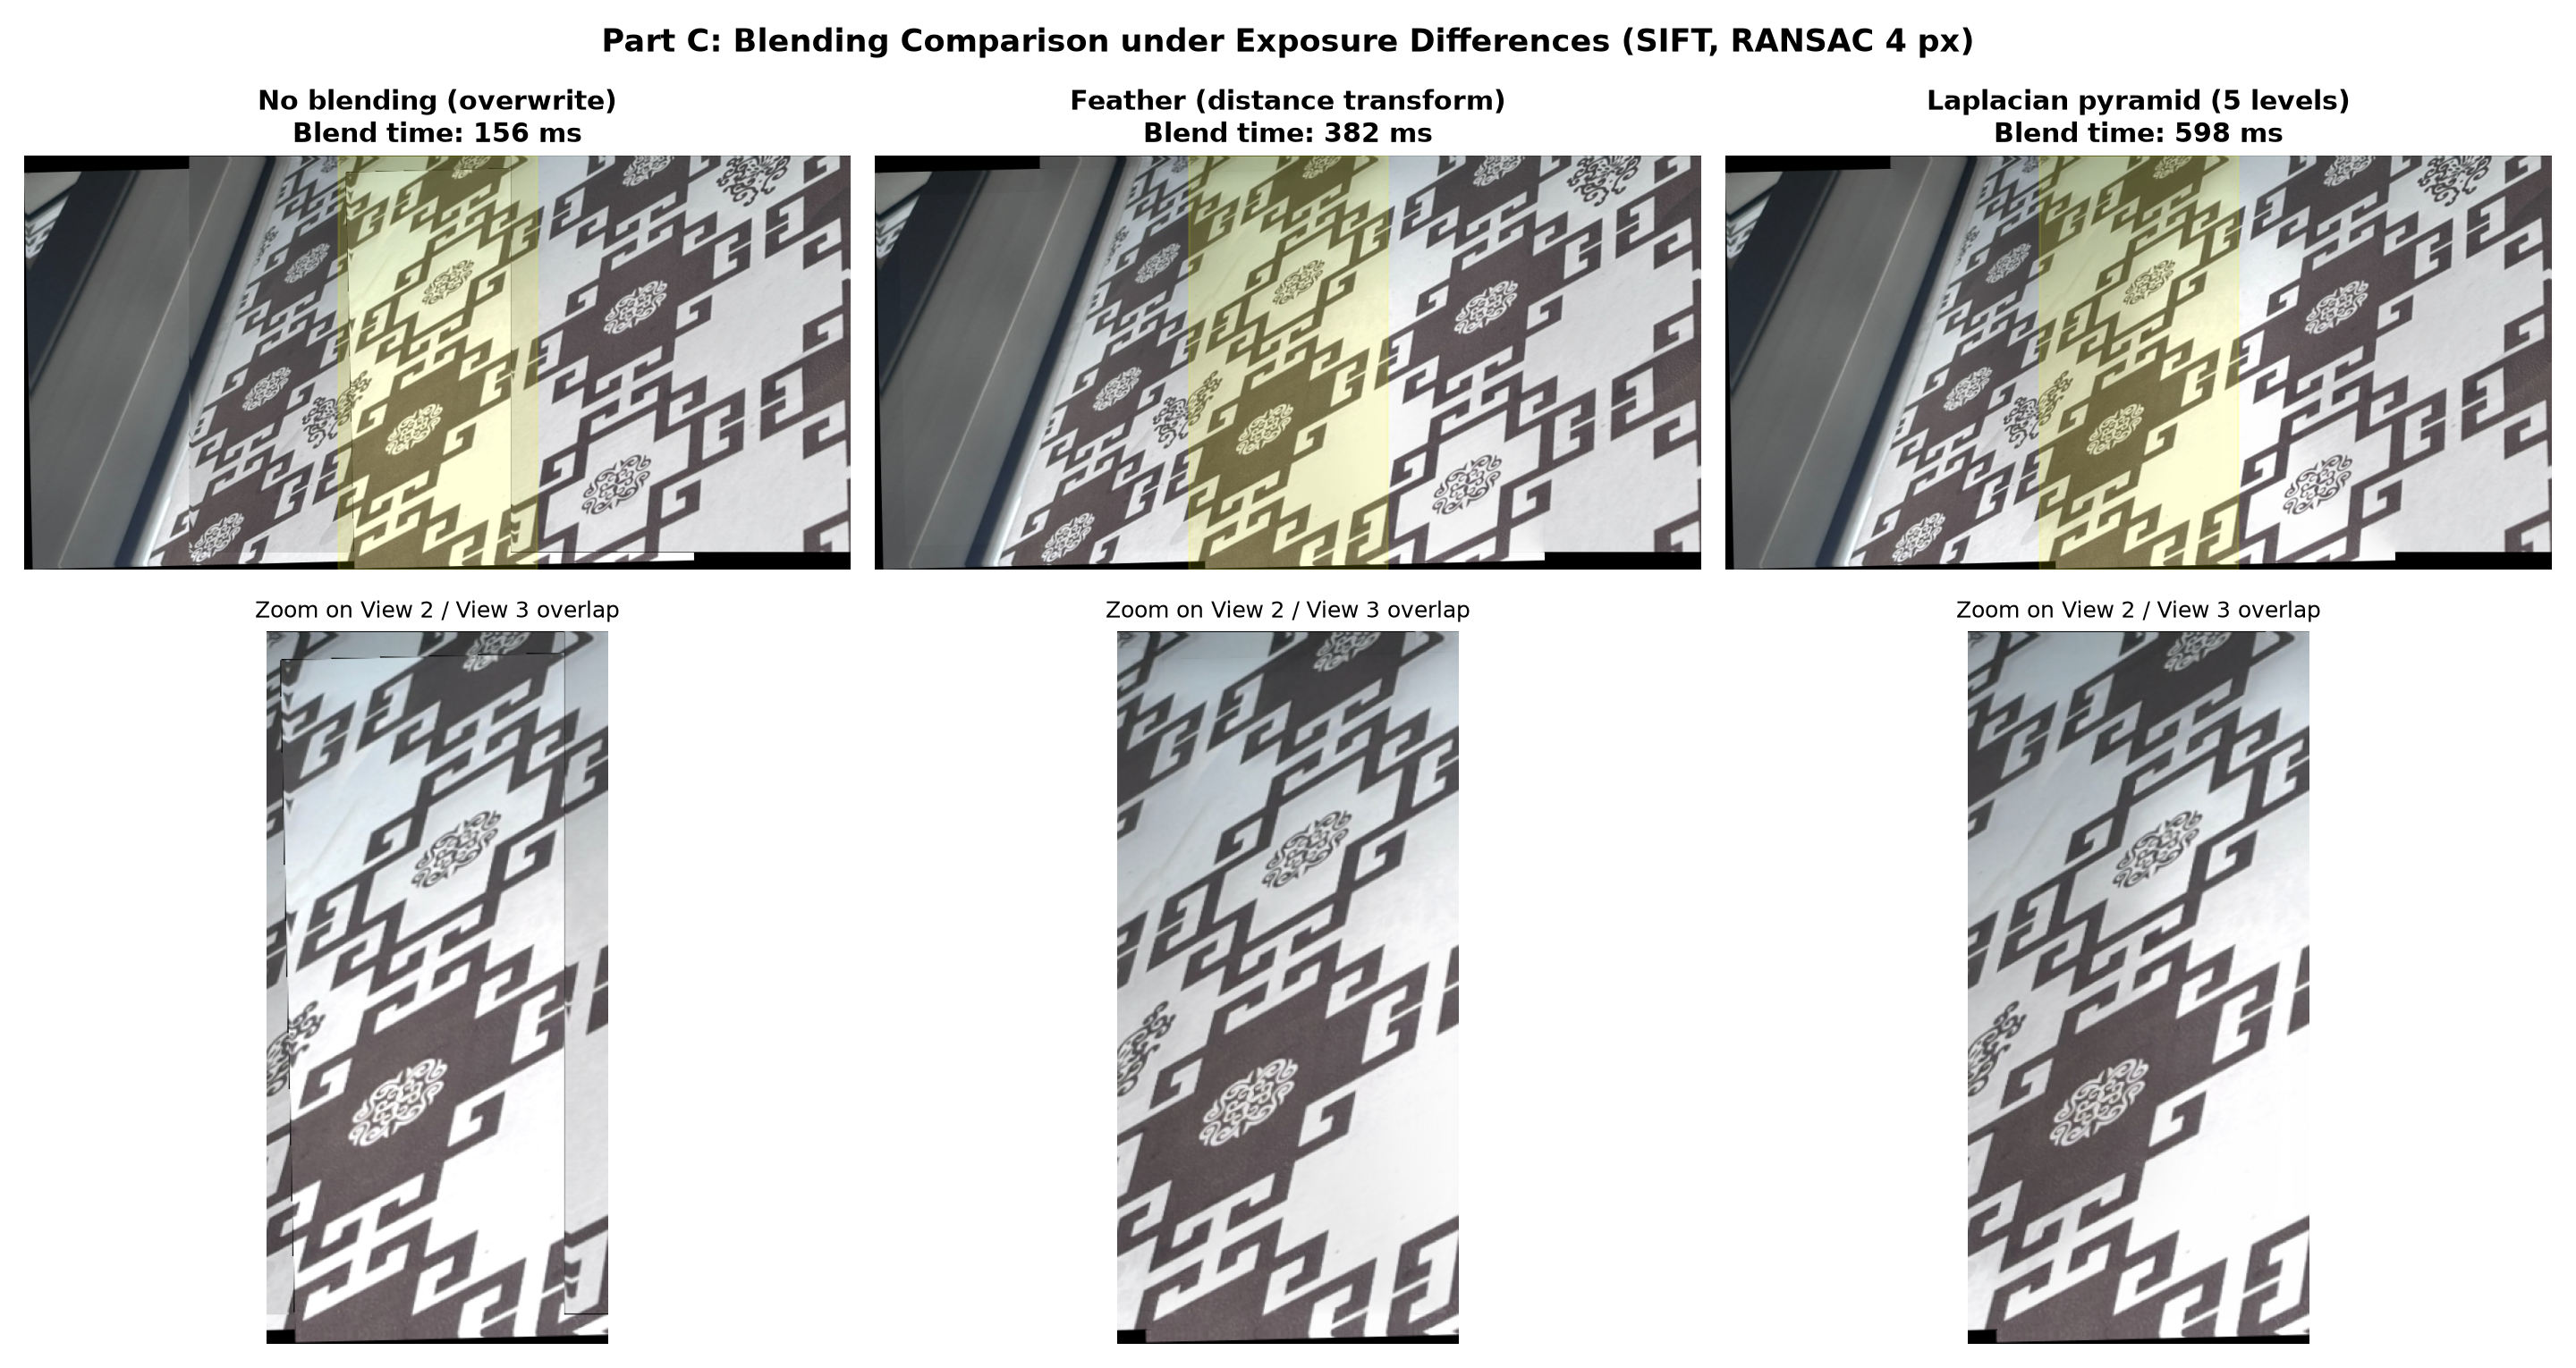
\includegraphics[width=\linewidth]{figures/blending_comparison.png}
    \caption{Panoramas without blending, with feathering and with Laplacian pyramid blending; bottom row zooms on the view 2/3 overlap where the exposure jumps from 0.88 to 1.10.}
    \label{fig:blend}
\end{figure}

\textbf{Quantitative analysis.}
\begin{itemize}[leftmargin=*]
    \item \textbf{Keypoints and matches:} the keypoint column sums both images of all three pairs
          (six detections). ORB returns the most keypoints ($\approx$2\,930 per image, close to its cap
          of 3\,000) and the most matches and inliers; SIFT finds $\approx$1\,660 and AKAZE the fewest
          ($\approx$1\,190 per image), but AKAZE keeps a comparable inlier ratio. As
          Figure~\ref{fig:kps} shows, ORB keeps only the 3\,000 strongest Harris-ranked corners, which
          cluster densely on the high-contrast ornaments in the centre and leave the image periphery
          almost empty; SIFT and AKAZE spread their keypoints much more evenly over the pattern
          corners and the whole view, which gives better-conditioned homography estimates.
    \item \textbf{Accuracy:} SIFT (0.23--0.27\,px) and AKAZE (0.26\,px) are about four times more accurate
          than ORB (0.87--0.99\,px). SIFT and AKAZE localize keypoints with sub-pixel refinement in a
          scale space, while ORB uses integer FAST corners on a coarse pyramid.
    \item \textbf{Inlier ratio:} 58--73\% for all detectors. The strongly repetitive wall pattern
          produces many plausible but wrong matches that the ratio test cannot reject, which RANSAC
          then removes.
    \item \textbf{RANSAC threshold:} raising the threshold from 2 to 4\,px adds inliers (ORB +99, or
          +3.4 points of inlier ratio) but also raises RMSE, since less accurate correspondences are
          accepted. For accurate detectors like SIFT the threshold hardly matters (+3 inliers).
    \item \textbf{Runtime:} SIFT is the slowest pipeline (813--883\,ms) because of its floating-point
          scale space and 128-D L2 matching; ORB (547--781\,ms) and AKAZE (715\,ms) are faster thanks
          to binary descriptors and Hamming distance. Warping and blending of the panorama canvas
          take 280--430\,ms of the total, so the end-to-end difference between detectors is smaller
          than the difference in feature extraction alone. Single-run timings vary by roughly
          $\pm$20\%, so only the ordering should be relied on.
\end{itemize}

\textbf{Qualitative analysis.}
\begin{itemize}[leftmargin=*]
    \item \textbf{Geometric alignment:} all three detectors give globally consistent panoramas, and
          even under zoom the pattern edges in the overlaps show no visible doubling (ghosting). ORB's
          higher RMSE ($\approx$1\,px) is below what is visible on this scene, so for this planar
          scene all three are adequate; the difference would matter for larger images or longer
          homography chains where errors accumulate.
    \item \textbf{Seams and illumination:} without blending, the exposure changes produce hard
          vertical seams and visible frame borders (Figure~\ref{fig:blend}). Feathering removes the
          seams but spreads the exposure change over the whole overlap, and any misalignment shows as
          ghosting. Laplacian pyramid blending gives the most natural transition: brightness is
          equalized smoothly while edges remain sharp, at about 1.6 times the blending cost of
          feathering (Table~\ref{tab:blend}).
    \item \textbf{Perspective distortion:} the wedge-shaped black borders at the panorama corners show
          how each view's perspective warp is undone when it is mapped into the plane of view 2.
          Views 1 and 4 are reached through one and two chained homographies, so any error in
          $H_{4\to3}$ propagates into $H_{4\to2}$. For wider panoramas, a cylindrical projection or
          bundle adjustment would be needed to limit stretching at the ends.
\end{itemize}

%=====================================================================
\section{Conclusion and Future Work}\label{sec:conclusion}
%=====================================================================
The experiments confirm that the best classical method depends on the noise or scene model. For
impulse noise, the non-linear median filter is far better than any linear filter, whereas for
Gaussian noise small Gaussian kernels give the best PSNR and moderate smoothing gives the best
SSIM; Laplacian sharpening improves perceived sharpness but must follow denoising. In stereo,
SIFT + RANSAC yields a sub-pixel fundamental matrix, and SGBM's global smoothness term produces
denser and about 43\% more accurate disparity than local Block Matching for a 2--3$\times$ runtime
cost, while being much less sensitive to block size. In stitching, SIFT and AKAZE give the most
accurate homographies, ORB is the fastest but least precise, and Laplacian pyramid blending best
hides exposure differences.

\textbf{Limitations and future work.} The stereo pair and multi-view images are synthesized
from one photograph so that exact ground truth is available; the next step is to capture a
calibrated real stereo pair (e.g.\ with \texttt{cv2.stereoCalibrate} and rectification) and to
evaluate on the Middlebury benchmark. Other improvements include edge-preserving filters (bilateral,
non-local means), left-right consistency checks and WLS filtering for disparity maps, gain
compensation and bundle adjustment for stitching, and seam finding via graph cuts.

%=====================================================================
\section*{References}
\addcontentsline{toc}{section}{References}
%=====================================================================
\begin{enumerate}[label={[\arabic*]}, leftmargin=*]
    \item R.~Szeliski, \emph{Computer Vision: Algorithms and Applications}, 2nd ed., Springer, 2022.
    \item R.~Hartley and A.~Zisserman, \emph{Multiple View Geometry in Computer Vision}, 2nd ed., Cambridge University Press, 2004.
    \item R.~C.~Gonzalez and R.~E.~Woods, \emph{Digital Image Processing}, 4th ed., Pearson, 2018.
    \item Z.~Wang, A.~C.~Bovik, H.~R.~Sheikh and E.~P.~Simoncelli, ``Image quality assessment: from error visibility to structural similarity,'' \emph{IEEE TIP}, 13(4), 2004.
    \item H.~Hirschm\"uller, ``Stereo processing by semiglobal matching and mutual information,'' \emph{IEEE TPAMI}, 30(2), 2008.
    \item D.~G.~Lowe, ``Distinctive image features from scale-invariant keypoints,'' \emph{IJCV}, 60(2), 2004.
    \item E.~Rublee, V.~Rabaud, K.~Konolige and G.~Bradski, ``ORB: an efficient alternative to SIFT or SURF,'' \emph{ICCV}, 2011.
    \item P.~F.~Alcantarilla, J.~Nuevo and A.~Bartoli, ``Fast explicit diffusion for accelerated features in nonlinear scale spaces,'' \emph{BMVC}, 2013.
    \item M.~A.~Fischler and R.~C.~Bolles, ``Random sample consensus,'' \emph{Communications of the ACM}, 24(6), 1981.
    \item P.~J.~Burt and E.~H.~Adelson, ``A multiresolution spline with application to image mosaics,'' \emph{ACM TOG}, 2(4), 1983.
    \item OpenCV documentation, \url{https://docs.opencv.org/4.x/}.
\end{enumerate}

\appendix
\section{Appendix: Python Code}
Full source code and results: \url{https://github.com/Habuck/computer-vision}.

\subsection{Part A: Image Filtering}
\lstinputlisting{../part_a_filtering.py}

\subsection{Part B: 3D Reconstruction}
\lstinputlisting{../part_b_stereo_3d.py}

\subsection{Part C: Image Stitching}
\lstinputlisting{../part_c_stitching.py}

\end{document}
